\chapter{Permissionless Consensus and Proof-of-Work}
\section{Permissionless Consensus}
\noindent
\textbf{Recap of the permissioned setting.} Thus far we've been studying consensus protocols
in the safe confines of the permissioned setting, in which the nodes running the protocol
are fixed and known in advance. This scenario made perfect sense when computer science
researchers started developing a theory of consensus protocols in the 1980s when a typical
application might be something like database replication (with a single company buying a
bunch of nodes to each store a copy of the database in the interests of very high uptime).
Thus far, we’ve also been making a PKI (public key infrastructure) assumption. That
is, we’re assuming that secure signature schemes exist, that each node has its public-private key pair, and that all nodes’ public keys are known to all nodes at the beginning of
the protocol (with each node signing its messages and verifying signatures on all received
messages). This is a “trusted setup” assumption, meaning we just assume that all nodes’
public keys were somehow shared correctly in advance of the protocol’s commencement (just
as we assumed that all nodes somehow obtained a correct version of the protocol’s code).
This trusted setup assumption is also totally reasonable in our running example of database
replication by a centralized organization. Tendermint (Chapter 7) is a canonical example of a permissioned consensus protocol.\\

\noindent
\textbf{Open participation and permissionless protocols.} The most famous blockchain protocols, such as Bitcoin and Ethereum, do not operate in the permissioned setting. To viscerally appreciate this point, I encourage you to take a break from this chapter and spin up
on your laptop or desktop a full node that validates the Bitcoin or Ethereum blockchains.
These blockchains have been running for years and have no idea who you are, and yet you
can simply download software, sync your machine with the blockchain so far, and join the
party. This is obviously very different from the classical permissioned setting.
Remember in Chapter 1 when I described a mental model of a blockchain as a (virtual)
computer in the sky, with no owner or operator? Really what this meant was that this
computer has lots of operators (coordinated via a consensus protocol), and moreover, you
yourself can become one of these operators, if you wish. This is the vision of permissionless consensus, and it is perhaps the most radical and audacious conceit in the original Bitcoin protocol.\\

\noindent
\textbf{The challenges of permissionless consensus.} A permissionless consensus protocol has
an unknown and possibly ever-changing set of nodes running it, which would seem to throw
an immediate wrench into, for example, a Tendermint-style protocol. In Tendermint with
100 nodes, nodes will wait to collect and see evidence of 67 votes before proceeding with
any action. If you don’t know how many nodes are there, how do you know how many
votes to collect? Similarly, without knowing which nodes are running the protocol, how
would you ever implement the round-robin approach to leader selection (in Tendermint, or
in longest-chain consensus)?
It also makes sense to think about permissionless consensus protocols as operating via
broadcast channels—perhaps implemented via a gossip protocol in a free-to-join peer-to-peer
network—rather than point-to-point communication. So, we’ll imagine that whenever an
honest node sends a message, it automatically broadcasts the messages to all other nodes.
(We don’t want to impose any unjustified restrictions on what Byzantine nodes can do,
so we’ll continue to allow them to, for example, send conflicting messages to different sets of honest nodes.) Similarly, clients (in the sense of a state machine replication protocol) are assumed to submit their transactions via a broadcast channel that is listened in on by
all the nodes that are currently running the protocol. This “broadcast-only” communication restriction shouldn't bother you too much—if you go back over our pseudocode for the
Tendermint protocol in chapter 7, for example, you’ll see that the nodes are basically already communicating via broadcast messages, anyway (e.g., announcing or echoing quorum
certificates).\\
The dream of permissionless consensus is an ambitious one, and in light of the seeming
incompatibilities between the constraints of the permissionless setting and the consensus protocols that we've seen thus far, you’d be right to question permissionless consensus protocols
with provable guarantees could even exist!\\
Such protocols do exist, if they didn’t, there’d be no chapter series! but, we’ll need some
additional ideas. As mentioned, an immediate obstacle to implementing a BFT-type protocol
in a permissionless setting is the seeming impossibility of supermajority voting when the set
of voters is unknown. A second issue, relevant to both BFT-type protocols and longest-chain consensus, is how to select leaders (i.e., which node gets to propose the next block).
“Round-robin order” doesn't appear to make sense with an unknown and ever-changing set
of nodes. “Uniformly random selection” also doesn't seem to make sense—if there were 100
nodes, in each round a given node should be selected as a leader with 1\% probability. If there were 1000 nodes, it should be a 0.1\% probability. But if the protocol doesn't know how many nodes there are, how can it know the appropriate probability with which to select a node?

\section{Random Sampling and Sybil Attacks}
\subsection{Why Permissionless Random Sampling Is Useful}
The key idea for transforming both BFT-type and longest-chain consensus protocols into
permissionless protocols is a permissionless and easily verifiable method of random sampling
one of the nodes that are currently running the consensus protocol. Two skeptical (but related)
questions should come immediately to mind: (i) sample from which distribution over nodes,
exactly? (ii) in any case, how would you do that without knowing which nodes are running
the protocol? Let’s put these questions aside briefly and outline how such a subroutine that 
would allow us to translate our permissioned protocols to the permissionless setting.\\

\noindent
\textbf{BFT-type consensus.} Consider the Tendermint protocol, for example. Recall from Chapter 7 that, in each round of the protocol, a single leader node proposes a (new or inherited)
block and then the entire set of nodes casts and tracks (two stages of) votes for that round’s
block proposal. The idea is to use, in each round of the protocol, the assumed method of
random sampling a node once to select that round’s leader as well as $s - 1$ additional times
to select the rest of the “committee” of $s$ nodes (here $s$ is a parameter of the protocol, like
$s = 20$ or $s = 100$, and is independent of the actual and unknown number $n$ of nodes running
the protocol). The $s$ randomly selected nodes are then the nodes tasked with carrying out
the current round of the Tendermint protocol. (If a node is randomly selected more than
once for the committee, then each time it was selected, it gets one distinct vote.) In
effect, this approach uses the assumed random sampling method as a “wrapper” to reduce
permissionless consensus to permissioned consensus.\\

\noindent
\textbf{Longest-chain consensus.} The utility of a random sampling method is even more obvious
in the case of longest-chain consensus, where each block is proposed unilaterally by a round’s
leader and nobody votes (other than the implicit votes in each leader’s decision of which
previous block to extend). Here, there’s no need to select a committee. The assumed
random sampling method can be invoked once in each round to select that round’s leader
(corresponding to step (2a) of the pseudocode in chapter 8), who then unilaterally proposes
blocks and their predecessors (step (2b)).

\subsection{Challenge: Sybils}
Should a permissionless and verifiable method of random sampling even exist?
For example, how can you select a node uniformly at random without knowing the set of
possible candidates?\\
As an initial (bad) idea, imagine that we tried to implement uniformly random node sampling as follows:\\
\begin{enumerate}[label=(\roman*)]
    \item nodes register their public keys in a smart contract stored on the blockchain;
    \item whenever needed, the protocol selects one of the currently registered keys
uniformly at random. (Technically, the protocol would select one of the registered keys pseudorandomly, for instance, using the
lower-order bits of the hash of some seed. If nodes running the
protocol know what hash function and seed the protocol is using, then they will also automatically know
which of the registered public keys was selected.)
\end{enumerate}
For example, if the method is used to select a block proposer for a
round, then the other nodes know to ignore any block proposals for that round that are not
signed with the private key corresponding to the selected registered public key.\\

The glaring issue behind this approach is that, while it’s all fine and good to maintain a
list of public keys, the protocol still has no idea about the mapping from registered public
keys to actual physical nodes. A single Byzantine node could costlessly create thousands or
millions of public-private key pairs (just type ssh-keygen at a Unix prompt) and register
them all, in effect, masquerading as a huge number of distinct nodes. (By contrast, you can think of the PKI assumption in a permissioned setting as asserting that there is
a one-to-one correspondence between the public keys registered with the protocol and the nodes that are
running the protocol.) Then, if there were
(say) 99 honest nodes that each registered only once, the one Byzantine node would be
selected by the protocol as the block proposer almost every round!\\

Generally, in computer science, when someone talks about a Sybil attack, they usually
mean the manipulation of some protocol through the creation of lots of identities. Basically,
a single party masquerades as many. Sybil attacks show up in lots of parts of computer
science, not just in blockchains, but I hope it’s very obvious why Sybil attacks are a real
danger for any random sampling approach to permissionless consensus.
In general, deliberately creating multiple identities in a system is often called a Sybil
attack. Systems in which Sybil attacks do not help the attacker are called Sybilproof or
Sybil-resistant. The naive approach to random sampling above is not Sybil-resistant. This
does not, of course, automatically mean that all approaches to random sampling are likewise
doomed to fail. Could there be a Sybil-resistant method for randomly selecting one of the
nodes running a consensus protocol—a method where the probability of a node’s selection
is independent of how many identities they might hide behind?\\
The answer, while not at all obvious, turns out to be “yes.” There are multiple methods
for Sybil-resistant random sampling, and in this chapter series we’ll focus on the two that are
most widely used as of 2022:
\nt{\begin{center}
    \textbf{Dominant Approaches to Sybil-Resistant Random Sampling}
\end{center}
\begin{enumerate}
    \item Proof-of-work. (See Section 9.4 for details.) This approach samples a node
running the protocol with probability proportional to the total amount
of computational power that it contributes.
    \item Proof-of-stake. (See Chapter 12 for details.) This approach samples a
node running the protocol with probability proportional to the total
amount of cryptocurrency that it has locked up in a designated smart
contract.
\end{enumerate}
}
The point is that the quantity that governs a node’s probability of selection—the combined
computational power of all its identities, or the combined staked cryptocurrencies of all its
identities is independent of how many identities it has. This is the sense in which
proof-of-work and proof-of-stake are sybil-resistance methods.

\section{Consensus Protocols vs. Sybil-Resistance Mechanisms}
\noindent
\textbf{We are not the same.} We've talked at length about two types of consensus protocols (BFT-type and longest-chain), and this chapter and chapter 12 will talk about two approaches to
Sybil-resistance (proof-of-work and proof-of-stake). Consensus protocols and Sybil-resistance
mechanisms are very different concepts, and you should keep them separate in your mind.
Conflating them is a common and confusing mistake and will mark you as a newbie to the
technical foundations of blockchains.\\

For example, think back to the permissioned setting with the PKI assumption that we
focused on in chapters 2–8. Sybil-resistance is trivial in this setting, each node is simply
assumed to have a unique public key and no Sybil-resistance method was needed. On the
other hand, we had a lot to say about the various consensus protocols you could use in this
setting. In the permissionless setting, you now have two design decisions to worry about: (i)
what underlying consensus protocol to use? (ii) how to prevent Sybil attacks?\\

Said differently, the purpose of a blockchain’s consensus protocol is to decide, given the
blocks that have been proposed (and perhaps voted upon) by the protocol’s participants,
which blocks should be considered finalized (and in what order). As we've seen, there are
different approaches to this decision. In a BFT-type protocol, a block is finalized if and only
if it is accompanied by an appropriate quorum certificate. However, in a longest-chain protocol,
the block is finalized if and only if it is sufficiently deep on the longest chain. These two types of
protocols are very different, but both exist for the same purpose: to decide which
blocks have been finalized.\\

Sybil-resistance mechanisms address a different question—who has the privilege of proposing and voting on blocks in the first place? Again, this took care of itself in the permissioned setting (with the PKI assumption), where the protocol could hard-code the allowable voters
in a BFT-type protocol (namely, all permissioned nodes) and the method of leader selection
in a BFT-type or longest-chain protocol (e.g., round-robin or uniformly at random).

\nt{
\begin{center}
    \textbf{Consensus vs. Sybil-Resistance}
\end{center}
\begin{enumerate}
    \item Sybil-resistance. Decide which nodes have the privilege of participating,
at which times and in what roles.[In the permissioned + PKI setting, hard-coded into the protocol.]
    \item Consensus. Give the block proposals (and possibly votes) of the participating nodes, which ones should be considered finalized?
\end{enumerate}}

For example, a common rookie mistake is referred to as “proof-of-stake consensus.” This phrase
doesn't typecheck, because “proof-of-stake” refers to a sybil-resistance mechanism, not a
consensus protocol. It does make sense to speak about a proof-of-stake blockchain, meaning a permissionless blockchain protocol that uses proof-of-stake for sybil-resistance (and
something else for consensus). Proof-of-stake blockchains come in many flavors—many use
BFT-type consensus, a few use longest-chain consensus, and some use still other approaches
to consensus.\\

\noindent
\textbf{Pairing proof-of-work with longest-chain.} The discussion above makes it
crystal clear that consensus protocols and sybil-resistance mechanisms are two very different
things. Accordingly, if we focus on the two dominant methods of consensus (BFT-type and
longest-chain) and the two dominant methods of sybil-resistance (proof-of-work and proof-of-stake), we can mix and match to get four different possibilities (Figure 9.1). Many but not all of the leading blockchain protocols can be categorized as one of these four types.
Some use alternative approaches to consensus (e.g., Avalanche) and others use alternative approaches to
sybil-resistance (e.g., Chia). Are any of
the four possibilities better or more natural than the others?\\

It’s become increasingly clear over the past few years that there is a fairly natural pairing between the two approaches to consensus and the two approaches to sybil-resistance.
For proof-of-work, Nakamoto got it exactly right in the original Bitcoin protocol: it pairs
perfectly with longest-chain consensus and is largely
incompatible with BFT-type consensus protocols. (The basic issue is that undetectable fluctuations in the total computational power devoted to the
protocol can cause liveness failures, even in the synchronous setting.) Thus, given that Nakamoto had decided to use proof-of-work to overcome Sybil attacks, they had no choice but to invent a
new approach to consensus. You sometimes hear the combination of longest-chain consensus
with proof-of-work sybil-resistance referred to as Nakamoto consensus, and we’ll get into
the details of it starting in the next section. As of this writing, the only major blockchain
protocols that use Nakamoto consensus are Bitcoin and its forks (like Bitcoin Cash, Litecoin,
and Dogecoin).
\begin{figure}[h]
    \centering
    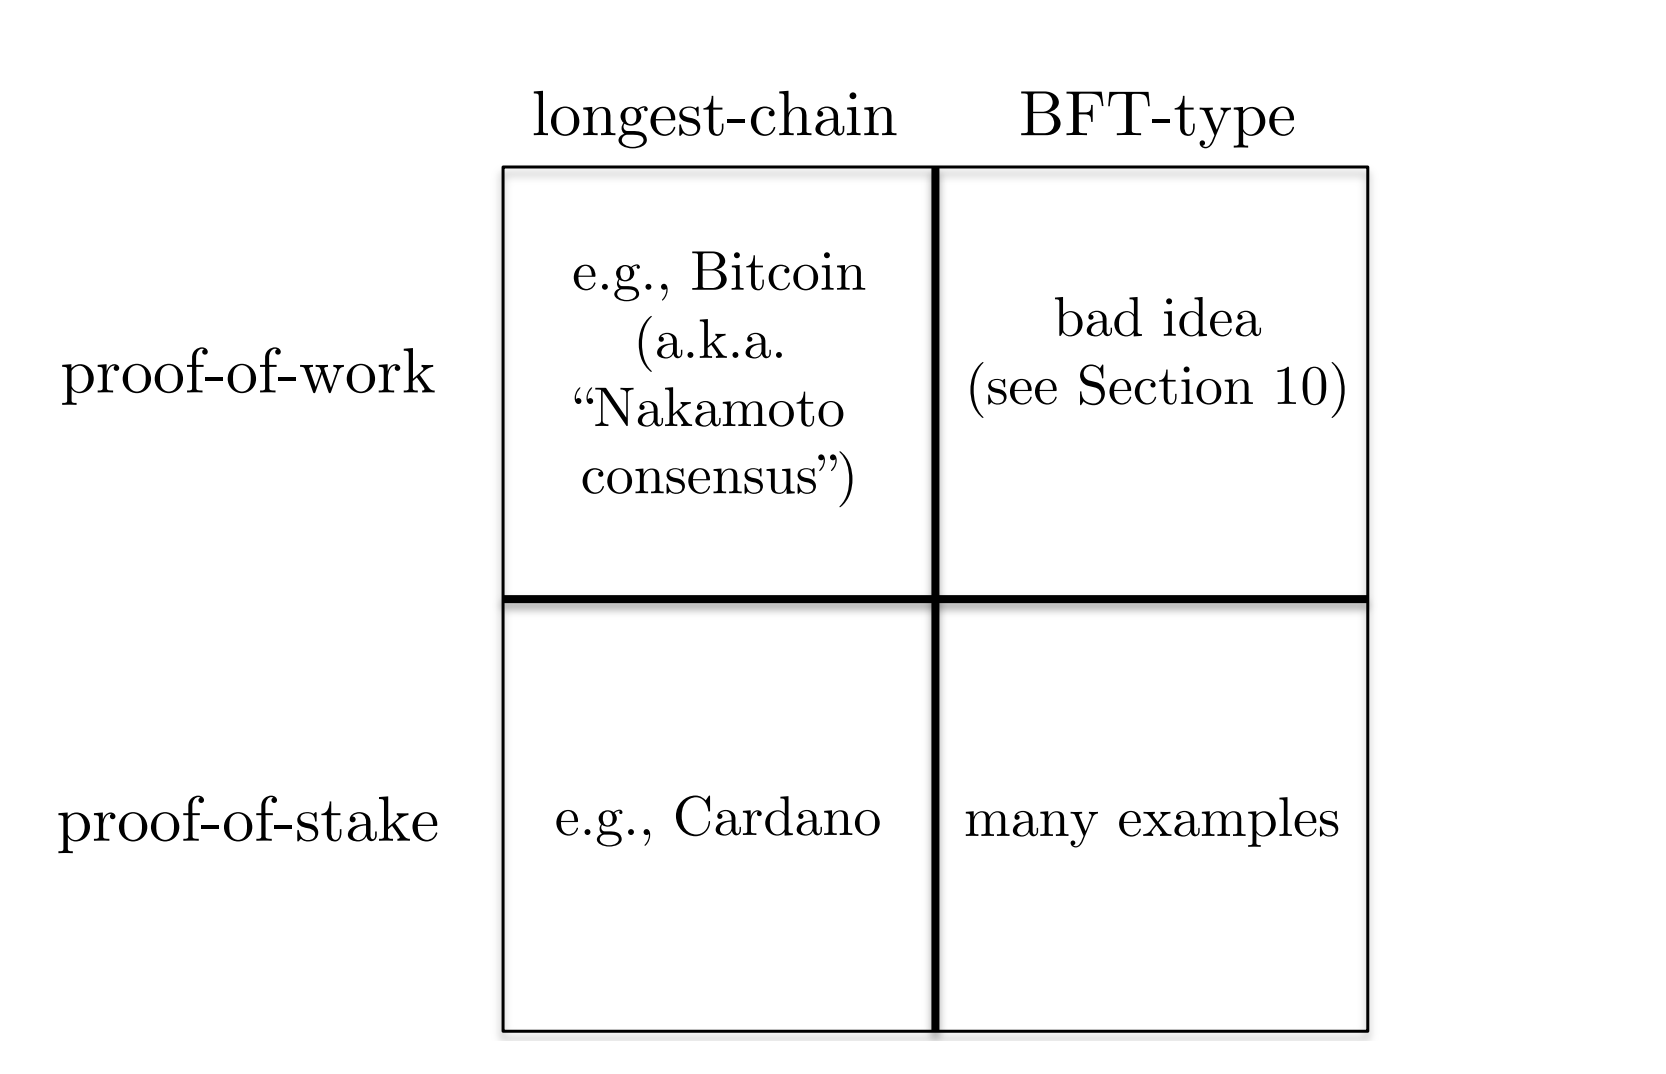
\includegraphics[scale = 0.5]{figures/f35.png}
    \caption{The two most common approaches to consensus and to sybil-resistance combine for
four categories that together capture many (but not all) of the leading “layer-one” blockchain
protocols.}
    \label{fig:mesh1}
\end{figure}\\
\noindent
\textbf{Pairing proof-of-stake with BFT-type consensus.} The story for proof-of-stake Sybil resistance is more nuanced. Most initial experiments with proof-of-stake attempted to use it
as a drop-in replacement for the proof-of-work part of the Bitcoin protocol. As we’ll discuss
in detail in Chapter 12, switching to proof-of-stake sybil-resistance causes a surprising number
of complications in longest-chain protocols. It’s not impossible to pull off a proof-of-stake
longest-chain protocol. There’s no impossibility result akin to the one in Section 12 for proof-of-work BFT-type protocols—but it’s a lot messier than you’d think. As of this writing, the
biggest (by market cap) proof-of-stake longest-chain blockchain protocol is Cardano.\\

The challenges of proof-of-stake longest-chain consensus design, along with the promise
of deterministic rather than probabilistic finality, have led to a shift in recent years toward
proof-of-stake BFT-type protocols (which at the time of this writing is the most common of
the four combinations among major “layer-one” protocols).\\

When you think about it, BFT-type protocols couple quite naturally with proof-of-stake
sybil-resistance. Arguably the most straightforward way to implement proof-of-stake-based
protocol participation is to require participants (identified by their public keys) to lock up
capital (in the form of the blockchain’s native cryptocurrency) in a designated smart contract
for a prescribed period of time. Once the participating public keys are known and publicly
visible in the staking contract, we are more or less in the permissioned setting (with public
keys playing the roles of nodes) with the PKI assumption. One can then run a BFT-type
protocol in which the participating “nodes” are the registered public keys; the voting power
of a registered public key should be proportionate to its stake so that no one can artificially and costlessly inflate their control over the protocol by creating a large number of public
keys. We’ll talk much more about the details and nuances of this approach in chapter 12.\\

\section{Proof-of-Work and Nakamoto Consensus}
For us, the main point of proof-of-work sybil-resistance will be to extend the permissioned
version of longest-chain consensus and its guarantees in chapter 8 to an analog (“Nakamoto
consensus”) in the permissionless setting.
\subsection{chapter 8 Recap}
We concluded Chapter 8 by isolating the properties of longest-chain consensus that were
really driving the analysis, and it’s worth recapping those here. Recall from that chapter
that the abstract description of longest-chain consensus includes an underspecified leader
selection step (step (2a)), in effect assuming that some mapping from rounds to rounds’
leaders is carried out by some black box (Figure 9.2). The first step is to start with a genesis block, which is known to all nodes at and only at the time of the
protocol’s commencement (a trusted setup assumption, called $"a1"$ in Lecture 8). The protocol proceeds in
rounds and in each round, there is a single leader node (selected in step $"a2"$ . In Step $"b2"$, the leader of the
round proposes blocks and explicit predecessors for those blocks. Honest nodes are instructed to propose a
single block that extends the longest chain that they are aware of, breaking ties arbitrarily.\\

\noindent
\textbf{Key properties for the analysis.} Three properties of this black box were necessary for
the proofs of the consistency and liveness properties in Chapter 8, none of which are
fundamental to the permissioned setting per se:
\nt{\begin{center}
    \textbf{Required Properties of the Leader Selection Box}
\end{center}
\begin{enumerate}
    \item (Same as assumption (A2) from chapter 8) It is easy for all nodes to
verify whether a given node is the leader of a given round.
    \item (Same as assumption (A3) from chapter 8) No node can influence the
probability with which it is selected as the leader of a round.
    \item (Required hypothesis for the common prefix property, liveness, and chain
quality guarantees in chapter 8) The sequence of leaders is sufficiently
balanced. (In longest-chain consensus, all honest nodes are interchangeable (they all behave identically) and all
Byzantine nodes are interchangeable (they are colluding anyway). Thus all that matters about a leader
sequence is its pattern of H’s and A’s.)
\end{enumerate}}\\

“Sufficiently balanced” means different things, depending on the context (see Chapter 8
for details), but there’s a single sufficient condition that guarantees (with high probability)
all of the variants that we care about:
\nt{\begin{center}
    \textbf{Key Sufficient Condition for Consistency and Liveness of
Longest-Chain Analysis}
\end{center}Leaders in different rounds are chosen independently and in each round, the
probability that the leader is Byzantine is at most $\alpha < \frac{1}{2}$.}

In other words, if you push the button on the black box to generate a new leader, the leader
that pops out is more likely to be honest than Byzantine (with each selection independent
of previous ones). This condition drove all the “proportional representation” arguments
that were used throughout Chapter 8, and given that the condition holds the consequent
arguments do not depend at all on being in the permissioned setting.\\
\begin{figure}[h]
    \centering
    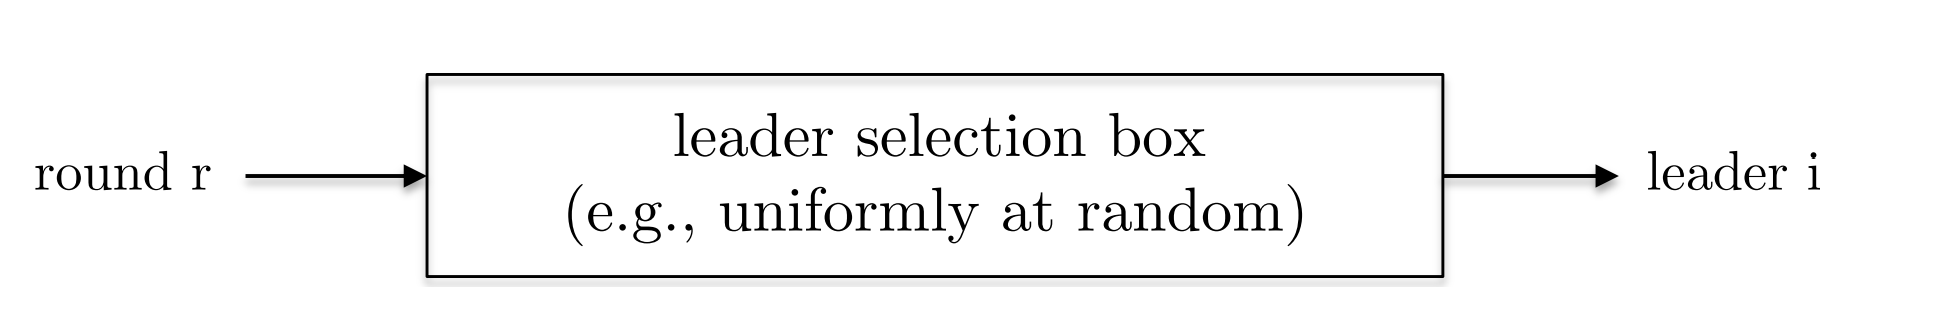
\includegraphics[scale = 0.5]{figures/f36.png}
    \caption{Step (2a) of longest-chain consensus is effectively a black box that maps round
numbers to leader nodes.}
    \label{fig:mesh1}
\end{figure}\\
\noindent
\textbf{The missing ingredient.} All the properties of longest-chain consensus that we care about
thus boil down to having a sufficiently balanced leader sequence, and this, in turn, boils down
to make sure that the key sufficient condition above holds. In the permissioned setting with
the PKI assumption, our solution was to assume that less than half the nodes are Byzantine
and to choose leaders independently and uniformly at random. For a permissionless solution,
we’ll need a different method of (sybil-resistant) random sampling (i.e., proof-of-work) and
a different assumption (that less than half of the total computational power is contributed
by Byzantine nodes). But as long as we manage to somehow satisfy the sufficient condition
above in the permissionless setting, we’ll be good to go, with all the consistency and liveness
guarantees from Chapter 8 carrying over (assuming, as usual, that the security parameter $k$
controlling the depth-til-finalization is chosen appropriately large).\\

In summary, the protocol and analysis of Chapter 8 is missing one and only one ingredient
from a permissionless protocol with the same consistency and liveness guarantees: a permissionless leader selection box that, under an appropriate assumption about the resources of
the Byzantine nodes, selects honest leaders more frequently than Byzantine ones. Section 9.4.2
next will supply exactly this missing ingredient.\\

\noindent
\textbf{Nakamoto consensus vs. abstract longest-chain consensus.} As an advance warning,
three aspects of the proof-of-work version of longest-chain consensus may surprise you, given
the abstract version that we've been focused on thus far. First, steps (2a) and (2b)—
the choice of a leader and that leader’s choices of blocks and block predecessors—will be
smooshed together into a single step, in effect with each node making its step (2b) choices
before knowing whether it’s selected as the round’s leader. Second, as we’ll see in Section 9.4.3,
the way the two steps will be smooshed together will prevent any leader from ever
proposing more than one block in a single round (i.e., as promised, assumption $"A4"$ from chapter 8 will be satisfied). Finally, you might be thinking of each round as having some fixed duration like 10 seconds. In the proof-of-work version of longest-chain consensus, new
rounds are triggered by random events and hence, a round’s duration is a random variable. By
contrast, none of these three idiosyncrasies are present in proof-of-stake versions of longestchain consensus (see Chapter 12).

\subsection{What Is Proof-of-Work?}
\noindent

`\textbf{The basic idea.} So how does "proof-of-work" work? The basic idea is to declare the
leader of the next round to be the first node that manages to come up with a solution to a
hard puzzle. It should seem plausible that, for an appropriate choice of puzzle, your likelihood
of being the first solver of the puzzle should depend on the total amount of computational
effort that you put into solving it (with the number of public keys that you control totally
irrelevant).\\
Even at this vague level of description, you should be able to see what we meant in chapter 8 when we stated that, in the proof-of-work version of longest-chain consensus, rounds are
“event-driven” (with the event being that some node successfully solves a hard puzzle). Likewise, you see why (as mentioned above) rounds will have variable and random durations (depending on whether some node gets lucky and finds a puzzle solution quicklyor not, or if all
nodes are unlucky and take a long time to find a puzzle solution).\\
In accordance with the permissionless setting and an unknown set of nodes, this approach
to randomly sampling a leader (with the leader whichever node happens to get lucky first)
is “bottom-up” (implemented by the nodes themselves through a process external to the
protocol) rather than “top-down” (implemented in protocol, as in the permissioned version
of longest-chain consensus).\\

\noindent
\textbf{A little history.} Proof-of-work actually dates back to 1992, seventeen years before the
Bitcoin protocol dropped. Dwork and Naor introduced the idea in the context of spam fighting, in order to ak the sending of an email modestly computationally expensive
(e.g., taking 0.1 second or 1 second per email on a commodity machine). This was a pretty
prescient paper, not only because blockchains didn’t exist yet, but (believe it or not) spam
email didn’t really exist yet either! Nakamoto and also Back’s later use
of the idea in HashCash was the first to apply the proof-of-work technique in the design
of consensus protocols. As of 2022, permissionless consensus is clearly the killer application
of proof-of-work.\\

\noindent
\textbf{Cryptographic hash functions.} What do I mean by a “hard puzzle”, the Saturday
New York Times crossword? One could imagine various approaches, but there’s one approach
that works really well. The same approach taken by Nakamoto in the original Bitcoin
paper, where the puzzle is to approximately invert what’s called a “cryptographic hash
function.”
To this point in the chapter series, we've adopted only one cryptographic assumption, 
the relatively uncontroversial assumption that secure digital signature schemes exist (see Chapter 1 for extended discussion). It’s possible to sign a message (using a private
key) such that anyone can verify the signature (using the corresponding public key), and such
that it’s impossible (for all practical purposes) to forge such signatures without knowledge of
the private key. As we've seen (e.g., in Tendermint), such signature schemes are very useful
in the design of (permissioned) consensus protocols (especially when all nodes’ public keys
are common knowledge at the start of the protocol, a.k.a. the PKI assumption).\\
Now we’re making a second cryptographic assumption—another one that is relatively uncontroversial in practice—namely that cryptographic hash functions (CHFs) exist. (5In this chapter, we’ll use CHFs only to implement proof-of-work sybil-resistance. Later in this course, they will be indispensable tools for a totally different reason, in the construction of cryptographic
commitment schemes (Merkle trees, etc.).) A hash
function, remember, is just a function from some domain to some range. Depending on
the context, hash functions can be used to compress or expand the input. In the context of
key-value stores implements as hash tables, the point of a hash function is to spread data
evenly throughout the hash table’s array (cf., “universal hashing”).\\
Cryptographic hash functions are designed with a different goal in mind, which is to
be totally inscrutable, meaning (for all practical purposes) totally unpredictable. Ideally,
whatever you feed in as input, you get back as output some intelligible gibberish that you’ve
never seen before in your life.\\
If you want to remember just one function that is believed to be cryptographic in this
sense, remember “SHA-256.” (Here “SHA” stands for “secure hash algorithm” and the
“256” refers to the number of bits of output. The input to SHA-256 can be of any length.)
I encourage you to look up a reference implementation of SHA-256 on the Web—it’s not
that long, maybe 100 lines of C code. Despite being a deterministic function whose source
code is known to everybody, it’s a totally inscrutable function. For all practical purposes,
the output of SHA-256 is completely unpredictable for any input that you haven’t already
evaluated it on.\\

\noindent
The random oracle assumption. We’ll formalize the idea of an inscrutable and unpredictable cryptographic hash function via the random oracle assumption. This assumption
will on the one hand be patently false, but in other ways a surprisingly close approximation
of reality. The assumption states that the hash function we’re using (such as SHA-256)
may as well be a random function, in the sense that no program that anyone writes will
ever be able to tell the difference. Here by “random function” we mean literally a function
chosen uniformly at random from the set of all functions with the given domain and range;
or, equivalently, a function for which the output of each input is chosen independently and
uniformly at random from the range (like $\{0, 1\}^{256}$).\\
I encourage you to think about a random function as being defined by lazy evaluation,
on a need-to-know basis. Think of it as a box with a little gnome in it. When you evaluate
the hash function $h$ for the first time on some input $x$, the gnome in the box flips a coin
256 (say) times and records and outputs the resulting string of 256 zeroes (heads) and ones
(tails).\\

If you ever re-evaluate the hash function at the same input $x$, the gnome in the box
checks its records and produces the same output $h(x)$ as before. But if you feed in some
different input $y$, the gnome in the box will flip a fresh set of 256 coins, recording and
outputting the resulting 256-bit string $h(y)$. It should be clear that such a function is
completely unpredictable—the only way to learn anything about its output on a given input
is to evaluate it on that input, and learning the outputs corresponding to a bunch
of inputs tells you nothing about the function’s outputs for other inputs.\\
The assumption that some concrete deterministic function is the same as a random
function is of course patently false. SHA-256, for example, is 100 lines of code, not a gnome
in a box. But here’s the thing: deterministic phenomena can appear random when there is
a bounded amount of computational power. For example, imagine you’re watching the coin
toss at the start of a sporting event, and you try to guess the outcome of the toss while the
coin is spinning rapidly while six feet up in the air. It’s hard to imagine how you would
predict the actual outcome with better-than-50\% probability. On the other hand, if you
had a much more computationally powerful system than just your naked eye, tons of cameras tracking the coin from different angles, a super-computer dedicated to fine-grained
physical simulations, etc.. It’s conceivable that you could predict the outcome of the coin
flip close to 100\% of the time. Similarly, while SHA-256 is in principle completely predictable
to a sufficiently powerful (but likely unrealizable) computer, it may well appear random to
any computation that we can realistically carry out.\\

There is also some chance that someone will come up with a new and practical algorithm
for better-than-random prediction of a concrete function like SHA-256, and such an event
would likely have detrimental consequences for proof-of-work blockchains like Bitcoin. Of
course, there’s also some chance that someone will come up with an efficient algorithm for
the factoring or discrete logarithm problems, in which case all hell will break loose (at least
in the short term). Just as we've been happy to assume that there’s no fast factoring or
discrete logarithm algorithm right around the corner, so too will we assume that better-than-random prediction of SHA-256 won’t happen anytime soon. This assumption grows more
battle-tested as the years roll by, and this is often all you can hope for when it comes to
cryptographic assumptions.\\

\noindent
\textbf{From CHFs to proof-of-work puzzles.} Now let’s take on faith that we have a concrete
function h like SHA-256 which is practically indistinguishable from a random function. How
can we use such a function to define hard puzzles? The canonical way is, given a “difficulty
threshold” $\tau$ :
\nt{\begin{center}
    \textbf{Canonical Proof-of-Work Puzzle}\\
    find an input $x$ such that $h(x) \leq \tau$.
\end{center}}
For concreteness, assume that the hash function h produces 256-bit outputs, which we then
interpret as nonnegative integers (written in binary).\\
The parameter $\tau$ is a tunable difficulty parameter. The hardest version of this puzzle is
when $\tau = 0$, in which case the task is to invert the function h at the all-zeroes output. The
easiest version is when $\tau = 2^{256}$, in which case every input qualifies as a solution. If $\tau = 2^176$ ,for example, the puzzle is to find an input $x$ such that h(x) has at least $(256 - 176) = 80$
leading zeroes. In general, bigger $\tau$ ’s mean easier puzzles (i.e., with more x’s qualifying as
solutions), and smaller $\tau$’s mean harder puzzles.
The fact that these types of puzzles have such precisely tunable difficulty is a big part of
why they form the basis for all proof-of-work blockchain protocols. For an NP-hard problem
like satisfiability or the traveling salesman problem, for example, it’s not at all clear what
it would mean to “double the instance difficulty.” (Whereas with the puzzles above, this
would mean cutting the value of $\tau$ in half.)\\
The optimality of repeated guessing under the random oracle assumption. Let’s
tie this section’s threads together by investigating the “partial CHF inversion” puzzles above
under the random oracle assumption. Suppose, for example, that we’re working with SHA256 and a difficulty threshold of $2^176$. The puzzle is then to find an input $x$ such that the
output of SHA-256 starts with 80 zeroes in a row.\\
Now let’s adopt the random oracle assumption, and model SHA-256 as a random function $h$—a gnome in a box. The game is now to find an input $x$ such that $h(x)$ starts with 80
zeroes—i.e., such that the first 80 coin flips by the gnome come up heads. Each time $h$ is
queried on a new input, there’s a one in $2^{80}$ chance that the first 80 coin flips are heads.
That is, the probability that any given input happens to be a puzzle solution is $2^{-80}$. Moreover, under the random oracle assumption, the only way you can learn anything about $h$
is through querying it at various inputs, and its outputs so far tell you nothing
about its outputs on as-yet-unevaluated inputs.\\
What this means is that, in searching for a puzzle solution, there are no options available other than repeatedly evaluating the hash function on some sequence of inputs $x_1, x_2, x_3, \cdots$ until you get lucky and stumble on an input $x_i$ with $h(x_i) \leq \tau$ . (You can
think of repeatedly throwing darts at a dartboard that has a small bullseye.)
And because each input is equally likely to be a puzzle solution (e.g., probability $2^{-80}$), your
probability of success is the same no matter what sequence of inputs you choose to evaluate
(as long as they are distinct).\\
With the parameter choices in our running example, it’s hard to find a
puzzle solution. With each guess having only a $2^{-80}$ of succeeding, you would expect to find
a puzzle solution only after trying $2^{80}$ different guesses (of course, it may be much more or
much less, depending on your luck). This would take forever on conventional computers, and
the only hope of ever finding a puzzle solution would be to throw an enormous amount of
specialized hardware at the problem (to explore the input space in a massively parallel
way). If $\tau$ were $2^{226}$, and so a success probability of $2^{-30}$ per guess, a commodity laptop
could find a puzzle solution without too much trouble.\\
To summarize: (i) if we assume that SHA-256 is indistinguishable from a random function, the only way to find a puzzle solution is through repeated guesses of distinct and
otherwise arbitrary inputs; (ii) if each guess is a puzzle solution with probability $p$, then on
average $\frac{1}{p}$ guesses are required to identify a solution. (Technically, this is that fact that the expected value of a geometric random variable with parameter $p$
(i.e., the number of coin flips requires to get a “head,” when the probability of heads is $p$) is $\frac{1}{p}$)\\

Whatever your doubts about the random oracle assumption, the upshot of the argument
above—that in a proof-of-work blockchain, nodes running the protocol will find puzzle solutions via naive repeated guessing is a remarkably accurate description of current practice.
\subsection{What Should Puzzle Solutions Encode?}
We now understand that, in the proof-of-work version of longest-chain consensus, the leader
of a round (step $"a2"$ in the abstract description) is defined as the first node to find a puzzle
solution, meaning identify an input $x$ such that $h(x) \leq \tau$ , where $h$ is a cryptographic hash
function (like SHA-256) and $\tau$ is a difficulty parameter (like $2^{176}$) that is somehow determined
by the protocol.\\

\noindent
\textbf{Committing to block proposals and predecessors.} Next, let’s drill down on the requirements for a puzzle solution $x$. Thus far, we've only required that it hashes to a sufficiently small number, but nothing’s stopping us from imposing some additional conditions,
for example requiring $x$ to conform to a prescribed format. Specifically, it will be convenient
to require $x$ to encode a node’s choices of blocks and predecessors in step $"b2"$ should the
node happen to be elected as the next leader—that is, should $x$ happen to hash to a number
that’s $\tau$ or less. Thus, a node will learn whether it’s the leader of the next round only after
it has committed to its step $"b2"$ choices and packaged them into an input x, under the
random oracle assumption, the node can’t predict whether $h(x) \leq \tau$ until it has actually
evaluated $h$ on $x$. (This is the “smooshing together” of steps $"a2"$ and $"b2"$ of longest-chain
consensus that was advertised in Section 9.4.1.) In the other versions of longest-chain consensus (the permissioned version in Chapter 8 and the proof-of-stake version in Chapter 12), by contrast, a leader is generally free to choose blocks and predecessors after it has been
selected as the leader of a round.\\

\noindent
\textbf{Forcing a single block proposal and predecessor.} But why stop there? In the abstract
description of longest-chain consensus, a round’s leader is free to propose multiple blocks.
(For example, a Byzantine node could propose one block to some of the honest nodes and a
conflicting block to the remaining honest nodes.) Meanwhile, the honest leaders are instructed
to propose only a single block (extending the longest chain). Given that we’re already
forcing a node to commit to its step (2b) choices in any candidate puzzle solution, why not
automatically disqualify any proposed input $x$ that names more than one block proposal?
In other words, let’s deem an input $x$ a puzzle solution if and only: (i) $x$ encodes a single
block proposal and predecessor; and (ii) $h(x) \leq \tau$. This makes it impossible for a leader
(Byzantine or otherwise) to propose multiple blocks in a single round. (This is the third
comment from Section 9.4.1, promising that the stronger assumption $"a4"$ from Chapter 8 would hold for Nakamoto's consensus.) Further proposals can be made only in future rounds
in which the same node is again the round’s leader. That requires solving an entirely new
puzzle; under the random oracle assumption, solving one puzzle provides no advantage to
solving a different one.\\

\noindent
\textbf{Format for puzzle solutions.} Conceptually, we can think of a candidate puzzle solution $x$ as having multiple fields. Two of the fields should contain a block proposal $B$ and a predecessor pred. You can also think of there being a third field that contains the node’s
public key "pk" (or at least, one of its public keys) so that the node can claim credit for the
puzzle solution. (The motivation for this will become obvious next chapter when we introduce cryptocurrency rewards
for block production. In practice, the public key of a round leader is included in its block only indirectly,
via what’s called a “coinbase transaction.”)\\

Summarizing, the tentative proposal to require inputs $x$ of the form $B||pred||pk$, where
“$||$” denotes concatenation. In addition to satisfying these formatting requirements, an input $x$ qualifies as a puzzle solution only if its hashes to something small (i.e., $h(x) \leq \tau$ ). We would therefore expect a motivated node running the protocol to experiment
with different $x$’s, i.e. with different blocks and/or different predecessors, and/or different
public keys that it can costlessly generate in its quest for a (properly formatted) input that
with a sufficiently small hash. Such experimentation is sometimes called grinding (as a node
is grinding through many candidate solutions, looking for a valid one).
Given nodes’ inevitable experimentation with different $x$’s, it’s convenient to include a
fourth field called a “nonce” (which stands for “number used once”). The nonce is just a
bunch of free bits with no purpose other than providing nodes with degrees of freedom for
generating lots of different well-formatted inputs (without needing to, for example, grind
over public-private key pairs).
\nt{
\begin{center}
    \textbf{Format for Puzzle Solutions}\\
    $B||pred||pk||nonce$
\end{center}}
Your mental model for a node running a proof-of-work blockchain protocol should be that it
fixes a block $B$ of transactions, a predecessor pred for that block, its public key $pk$, and then
grinds through nonces nonce until $h(B||pred||pk||nonce) \leq \tau$. (If it hears about a new block
in the meantime, produced by some other node, it will likely update its choices of $B$ and $pred$
and restart the nonce grinding process.) Technically, in proof-of-work blockchains like Bitcoin, one often differentiates between the nodes that
are grinding away and striving to be selected as a leader and to propose a new block (usually called miners,
as if digging for gold (i.e., block rewards)) and the nodes that are merely maintaining the blockchain and
checking that miners are following the protocol’s rules (usually called full nodes or validators). For example, if you’re building on top of a blockchain and want to query the blockchain’s state from a smart contract,
you care about talking to a validator, not a miner. For simplicity, we’re currently assuming that every node
running the protocol is acting as both a miner and a validator.
This is a surprisingly accurate description of how proof-of-work blockchains like Bitcoin work in practice.

\section{Properties of Proof-of-Work & Nakamoto Consensus}
Now that we understand how proof-of-work works, we can return to fulfilling our earlier
promises. This section proves that proof-of-work is indeed resistant to sybil attacks (under
the random oracle assumption), that it provides the missing “permissionless black box”
needed to extend longest-chain consensus from the permissioned to the permissionless model,
and notes some additional remarkable properties possessed by Nakamoto consensus.
\subsection{Sybil-Resistance}
The most important property of proof-of-work for our purposes is its sybil-resistance, meaning
that the probability that a node is selected as the next leader, i.e. is the first to solve a
hard puzzle, or specifically to partially invert a cryptographic hash function is independent
of the number of public keys that it might control.\\
For the analysis, we will adopt the random oracle assumption of Section 9.4.2—that whatever hash function we’re using (e.g., SHA-256) is indistinguishable from a random function,
in which a gnome in a box flips a fresh set of 256 coins every time a new input is evaluated. We will also assume that every node running the protocol repeatedly tries different
$nonces$ until some get lucky and finds a nonce that (coupled with the node’s choice of the block,
predecessor, and public key) hashes to a number that is at most the current difficulty threshold $\tau$.
23 As discussed in Section 9.4.2, under the random oracle assumption, this is the obvious
and optimal strategy for the nodes running the protocol.\\
Under these assumptions, the probability that a given node is selected as the next leader
depends only on the total amount of computational power that it contributes to the protocol,
independent of the number of identities it might control. Formally:\\
\thm{Sybil-Resistance of Proof-of-Work}{Suppose $n$ nodes $1, 2, \cdots , n$ make
$\mu_1, \mu_2, \cdots, \mu_n$ distinct nonce guesses per second. Then, for every node $i$ and round $r$,
$$\textbf{Pr}[\text{node $i$ is the round-$r$ leader}] = \underbrace{\frac{\mu_i}{\sum_{j=1}^n \mu_j}}_{\text{$i$’s fraction of
the overall hashrate}} \quad (1)$$
Moreover, the selections of leaders in different rounds are independent.}

The proof of Theorem 9.5.1 is just some easy probability that follows from the random oracle
assumption, as we’ll see below. Before that, a few comments. First, the $\mu_i$’s are often referred to as the nodes' hash rates, reflecting the fact that we care about a node’s “computational
power” only since we care about the rate at which it can try out different nonces
(which one hash function evaluation necessary and sufficient to check if a given choice yields
a valid puzzle solution). (For instance, the specialized hardware (ASICs, for “application-specific integrated circuits”) used for
Bitcoin mining are not general-purpose computers and are optimized to evaluate SHA-256 as quickly as
possible (at the expense of all other functionality).) Second, while the statement of Theorem 9.5.1 references a set
of $n$ nodes for notational purposes, we stress that the proof-of-work process works in the
permissionless setting and so is independent of what this node set might be. At any given
time, there will be some set of nodes running the proof-of-work protocol and searching for
puzzle solutions, those nodes will have some hash rates at that time, and Theorem 9.5.1 will
then apply to those particular nodes and hash rates at that time. By “node,” we mean an actual physical machine running the protocol, not a specific public key. For
example, if a node is capable of evaluating one billion nonces per second, this will be true whether all the
guesses are concentrated under a single pubic key or split 50/50 between two different public keys. Spinning
up multiple threads under different identities doesn't magically increase the number of guesses that the
machine can make. Finally, because the
right-hand side of (1) is independent of how many identities node $i$ controls, Theorem 9.5.1
implies that proof-of-work is indeed sybil-resistant.

\cor{Sybil-Resistance of Proof-of-Work}{The probability that a node is selected as a leader depends only on its share of the overall hashrate, independent of its number
of identities.}

Looking at Theorem 9.5.1 and Corollary 9.5.1, it should be clear that a node $i$ can increase
its probability of selection by beefing up its machine and increasing its hash rate $\mu_i$ (assuming
other nodes’ hash rates stay fixed, this would increase node $i$’s share of the overall hash rate).
But at least this is a costly manipulation (more computers \Rightarrow more money), unlike sybil
attacks, which are essentially costless (repeatedly enter ssh-keygen at a Unix prompt). You
might have mixed feelings about divvying up control over a blockchain protocol according to
the nodes’ financial investments in hash rate, but this (or something similar with a different
costly resource) appears to be necessary to achieve sybil-proofness in a permissionless setting.
The analysis. The proof-of-work sybil-proofness property (Theorem 9.5.1) may seem intuitive.
If one machine is making guesses twice at rapidly as another one, presumably it’s twice as
likely to be the first node to find a puzzle solution. If you find this argument convincing, feel
free to skip to Section 9.5.2. But given the importance of this property, it seems appropriate
to provide a more formal proof of it (under the random oracle assumption).\\

\noindent
\textit{Proof of Theorem 9.5.1:} Fix an arbitrary node $i \in \{1, 2, \cdots, n\}$. Consider two events (i.e.,
things that might or might not happen): event $A$, that a given guess was made by node $i$;
and event $B$, that a given guess turns out to be a valid puzzle solution (and therefore kicks off a new round). The theorem statement concerns the conditional probability $\textbf{Pr}[A|B]$—the probability that the guesser of a puzzle solution (i.e., the leader of round) is the node $i$.\\
Under the random assumption, every guess made by a node produces a fresh
string of perfectly random bits (the coin flips by the gnome in the box). This means that the
probability that any given guess is a valid puzzle solution is the same no matter which node
proposed it. (As all nodes face the same difficulty parameter $\tau$ .) In particular, event $B$ is
independent of event $A$: $\textbf{Pr}[B|A] = \textbf{Pr}[B]$. Independence of events is symmetric, to event $A$
must then be independent of event $B$: $\textbf{Pr}[A|B] = \textbf{Pr}[A]$. (Formally, this is a special case of
Bayes’ rule.) The probability $\textbf{Pr}[A]$ that the current guess was made by node $i$ equals the
relative frequency of guesses made by node $i$, which is $\frac{\mu_i}{\sum_{j=1}^n \mu_j}$, as promised.\\
Finally, under the random oracle assumption, puzzle-solving efforts from past rounds have
no bearing on future rounds (with all nodes continuing to repeatedly try out different guesses,
each equally likely to succeed). Thus, leaders of different rounds are selected independently.

\subsection{Permissionless Consensus with Provable Guarantees}
Supplying the missing ingredient. Now let’s segue from studying proof-of-work in its
own right and pick up the story where we left off at the end of Section 9.4.1, examining the
composition of proof-of-work sybil-resistance with longest-chain consensus (i.e., Nakamoto
consensus). Back in that section, we agreed that the key to the analysis in Chapter 8 (which
established several probabilistic consistency and liveness properties for longest-consensus)
was the property that leaders in different rounds are chosen independently and, in each
round, the probability that the leader is Byzantine is at most $\alpha < \frac{1}{2}$. This property drove
all the “proportional representation arguments” that implied (with high probability) various
balancedness properties of the generated leader sequence, and these balancedness properties
in turn implied the consistency and liveness guarantees (provided the security parameter $k$
is chosen sufficiently large, given the bound $\alpha$ on the probability of a Byzantine leader and
the duration of interest). We barely used the power of the permissioned model in these
arguments only for implementing the leader selection black box, e.g. using a round-robin
order or uniformly random leaders.\\
In Nakamoto consensus, rounds’ leaders are chosen using proof-of-work (with the leader
of the next round the first node to partially invert a cryptographic hash function, and with
their proposed block and predecessor encoded in the solution). Proof-of-work supplies the
missing permissionless ingredient and turns longest-chain consensus is to a purely permissionless consensus protocol—the protocol operates without any knowledge of the set of nodes (with the nodes themselves rather than the protocol selecting leaders, in effect) and with all
communication via broadcast. The sybil-resistance property of proof-of-work (Theorem 9.5.1)
implies that the probability that a given node is the leader of a given round equals its share
of the overall hash rate, with leaders of different rounds chosen independently. By extension,
the probability that the leader of a given round is a Byzantine node equals the fraction of
the overall hash rate that is controlled by such nodes. Thus, as long as this fraction $\alpha$ is less
than $\frac{1}{2}$, we should be good to go! (This < 50\% Byzantine hash rate assumption replaces our
old assumption from the permissioned model of < 50\% nodes.)\\

\noindent
\textbf{Checking the assumptions.} Some chores remain before we can declare victory with
a permissionless consensus protocol with provable guarantees. Specifically, the analysis of
longest-chain assumption relied on five assumptions (above and beyond the permissioned
model and the PKI assumption), and we need to check that our proof-of-work implementation
of longest-chain consensus doesn't violate any of them so that that chapter’s analysis continues
to apply to Nakamoto consensus. For reference, here’s a restatement of those assumptions
from Chapter 8:
\nt{
\begin{center}
    \textbf{Assumptions (A1)–(A5)}
\end{center}
\noindent
(A1) No node has knowledge of the genesis block prior to the deployment of
the protocol.\\
\noindent
(A2) It is easy for all nodes to verify whether a given node is the leader of a
given round.\\
\noindent
(A3) No node can influence the probability with which it is selected as the
leader of a round in step (2a).\\
\noindent
(A4) Every block produced by the round-$r$ leader must claim as its predecessor
some block that belongs to a previous round.\\
\noindent
(A5) At all times, all honest nodes know about the exact same set of blocks
(and predecessors).}

\noindent
\textbf{Assumption (A1).} Let’s take them one at a time. Assumption (A1) was important in
our proof in chapter 8 of the common prefix property. It is a trusted setup assumption.
Basically, that Byzantine nodes couldn't get started on puzzle-solving until the protocol was
deployed, meaning that it’s the responsibility of whoever deploys the protocol rather than
that of the protocol itself. Thus, in our analysis, we simply assume that it's true without
worrying about why.\\
That said, in practice, when deploying a protocol, one can take pains to build up confidence among participants that the trusted assumptions are indeed true. Nakamoto was
well aware of Bitcoin’s trusted setup assumption, and released the protocol (on January 3rd,
2009) with a genesis block that included a hard-coded message that referenced a very recent
headline of the Financial Times (about a bailout for British banks—remember this was in the
middle of the Great Recession). Presumably, no one (not even Nakamoto) knew what
the Bitcoin protocol’s genesis block was until at most a few hours before its deployment.\\

\noindent
\textbf{Assumption (A2).} The next three assumptions are asserted properties of the protocol
(as opposed to an external-to-protocol trusted setup assumption), we need to check that
all of them hold. Happily, with proof-of-work sybil-resistance and with puzzle solutions
encoding block proposals and predecessors, these all take care of themselves. Let’s start with assumption (A2). A round’s leader is defined as having a valid puzzle solution. If
a node can exhibit such a solution (an input $x$ that is formatted correctly and with $h(x) \leq \tau$ ),
all the other nodes can check its formatting and check for itself that it hashes to something
small. (The hash function $h$ is part of the protocol’s description and designed to be easy
to evaluate, and as we’ll see in Section 9.6, any node following along with the protocol knows
what the current difficulty parameter $\tau$ is.) Thus if you possess such a puzzle solution, all
other nodes can easily recognize you as the next leader. If you don’t, there’s no way to trick
the other nodes into thinking that you are the next leader (whatever you try to supply to
them will either be improperly formatted or hash to something bigger than $\tau$, so you’ll be
caught red-handed by the other nodes).\\

\noindent
\textbf{Assumption (A3).} Assumption (A3) follows immediately from the sybil-resistance property of proof-of-work (Theorem 9.5.1, which relies on the random oracle assumption). The
probability that a node is selected as a round’s leader equals its fraction of the overall
hash rate, and there’s nothing that the node can do about it. (Other than investing in additional hashing power, which occurs at a slower timescale than the one we’re
analyzing here; see also the discussion following Corollary 9.5.1. This assumption (A3) might more accurately
state that no node can costlessly influence the probability with which it is selected as the leader of a round.)

\noindent
\textbf{Assumption (A4).} For assumption (A4), as advertised, Nakamoto consensus 
satisfies the stronger condition (A4’) that at most one block is produced in each round. This
follows from the fact that there is exactly one puzzle solution per round (by the definition
of a round) and that a valid puzzle solution can (by definition) name only a single block
proposal (see Section 9.4.3). Also, such a puzzle solution can only name as a predecessor a
block that existed at the time of its creation, which must necessarily have been produced in
some previous round.\\

\noindent
\textbf{Assumption (A5).} The final assumption (A5) is an assumption about the communication
network (that communication is instantaneous), not the protocol, and so we’re not in a
position to enforce it. The good news is that this assumption isolated the most difficult
aspect of consistency in longest-chain consensus which is finality, also known as the consistency of a node
with its future self (as opposed to consistency between nodes at a given moment in time,
which is trivialized by (A5)). The bad news is that this assumption is false, even
in a well-functioning network, messages have nonzero delays. We’d therefore like to relax
this assumption to something more plausible—at the very least, to the synchronous model
with some nonzero maximum message delay $\Delta$—without materially changing the consistency
and liveness guarantees that we've come to expect for longest-chain consensus. And this is
exactly what we’ll do in Section 9.7 (under the assumption that $\Delta$ is small relative to the
expected duration of a round)!\\

\noindent
\textbf{Nakamoto consensus: the final scorecard.} Summarizing, here are the key assumptions under which Nakamoto consensus has provable (probabilistic) consistency and liveness
guarantees:
\nt{
\begin{center}
    \textbf{Key Assumptions for Consistency and Liveness of Nakamoto Consensus}
\end{center}
\begin{enumerate}
    \item The security parameter $k$ is sufficiently large.
    \item The random oracle assumption—e.g., SHA-256 is for all practical purposes indistinguishable from a random function (see Section 9.4.2).
    \item The trusted setup assumption (A1), no advance knowledge of the genesis block.
    \item Less than half of the hash rate is controlled by Byzantine nodes (by Theorem 9.5.1, this guarantees that the key sufficient condition from Chapter 8
is satisfied). [Actually, in the general synchronous model this degrades slightly; see Section 9.7.4]
    \item The communication network conforms to the synchronous model, with
finite maximum message delay $\Delta$.
    \item The difficulty parameter $\tau$ is tuned so that the average duration of a
round (i.e., the average amount of time between two successive valid
puzzle solutions) is much larger than $\Delta$. [How much larger? Think 1–2 orders of magnitude. The precise bound on the maximum-allowable fraction of Byzantine hash rate depends on the ratio between the average round duration and $\Delta$, and approaches
50\% as this ratio approaches infinity (see Section 9.7 for details).]
\end{enumerate}
}

The next two sections (Sections 9.5.3 and 9.5.4) discuss some additional remarkable properties
of Nakamoto consensus; the time-constrained reader can skip to Section 9.6 without any loss
of continuity.
\subsection{How Did We Elude the PSL-FLM Impossibility Result?}
\noindent
\textbf{Strong permissionlessness.} While Nakamoto consensus does require a trusted setup
assumption—assumption (A1), that no node has advanced knowledge of the protocol’s genesis
block—it does not require our usual trusted setup assumption, the PKI assumption. That
is, nodes running the protocol require no knowledge of the public keys possessed by the
other nodes running the protocol. For example, to join the set of nodes running the Bitcoin
protocol, all you need to do is download some software, sync up your machine to the current
state of the blockchain, and start following along (maintaining the blockchain, trying to find
puzzle solutions, etc.). No one else knows that you exist!\\
While there’s no single widely accepted definition of a “permissionless” protocol, no
matter what definition you use, the Nakamoto consensus certainly qualifies. At any moment
in time, a new block might well get produced under a public key that nobody has ever
seen before. (Once that block is published, everybody sees the public key responsible for
it. But whoever published the block can generate and switch to using a new public key
immediately, thereby returning to puzzle-solving in complete obscurity.) As we’ll see in
Chapter 12, blockchains based on proof-of-stake sybil-resistance tend to be “somewhat less
permissionless,” in that the set of public keys eligible for producing the next block is usually
maintained in public view (i.e., the set can be derived from the blockchain’s current state).\\

\noindent
\textbf{Review: the PSL-FLM impossibility Result.} If you’ve been following this chapter
series closely, you might at this point have a question, namely: Why doesn't
Nakamoto consensus contradicts the impossibility results for SMR protocols that we saw
earlier in the series.\\
Back in chapter 2, we studied the Dolev-Strong protocol, which solves the Byzantine
broadcast problem (satisfying termination, validity, and agreement) even when 99\% of the
nodes are Byzantine, under two key assumptions: (i) the synchronous model; (ii) the PKI
assumption. (Iterating this protocol then gave us an SMR protocol satisfying consistency and
liveness.) Later chapters probed to what extent assumptions (i) and (ii) are necessary for this
result. For example, in chapter 6 we saw that, in the partially synchronous model, there’s
no solution to the Byzantine broadcast problem when at least one-third of the nodes are
Byzantine (even with the PKI assumption).\\
Relevant here, though, is our probing of assumption (ii) in Chapter 3. Let's flashback the thought experiment on the hexagon and the various ways
that a Byzantine node might simulate simultaneously four fictional honest nodes. It stated
that without the PKI assumption, even in the synchronous model and even assuming that
cryptography exists, no protocol solves the Byzantine broadcast problem when
at least one-third of the nodes are Byzantine. Thus, the advance distribution of nodes’ public
keys was an unavoidable requirement of the Dolev-Strong protocol.\\
Meanwhile, Nakamoto consensus can solve the state machine replication (SMR) problem
even when more than one-third (up to 49\%) of the hash rate is Byzantine. Why doesn't this
guarantee (without PKI, consensus is possible with 49\% Byzantine) contradicts the PSL-FLM
impossibility result (without PKI, consensus is impossible with 34\% Byzantine)?\\

\noindent
\textbf{Some false resolutions.} The answer is subtle, so let’s step through some incorrect answers
before arriving at the correct resolution.\\

\textit{Guess \#1: the PSL-FLM impossibility result only limits the fraction of nodes that are
Byzantine, while the Nakamoto consensus guarantees require that less than half the
hash rate is controlled by Byzantine nodes.}\\

The “node versus hash rate” distinction is irrelevant. Our guarantees for Nakamoto consensus
hold for any distribution of hash rates (as long as less than half of the total is controlled by
Byzantine nodes), so they hold in particular when every node happens to have the
same hash rate. In this special case, the “< 50\% hash rate” assumption becomes a “< 50\%
nodes” assumption, which would seem to contradict the one-third threshold established by
the PSL-FLM impossibility result.\\

\textit{Guess \#2: the PSL-FLM impossibility result is for the Byzantine broadcast problem,
while the Nakamoto consensus protocol solves the SMR problem.}\\

This is a better guess, but still incorrect. The hexagon argument from Chapter 3 can in
fact be extended to hold also for the Byzantine agreement and SMR problems (see the
Appendix of that chapter). Alternatively, Nakamoto consensus can be extended to solve the
Byzantine agreement problem when 49\% of nodes/hash rate are Byzantine (even without the
PKI assumption).\\

\textit{Guess \#3: the PSL-FLM impossibility result is for deterministic protocols that guarantee safety and liveness, while the Nakamoto consensus protocol is randomized and
guarantees only probabilistic safety and liveness.}\\

It's another good guess, but again not the correct resolution. As it turns out (an excellent
tricky homework problem), the proof of the PSL-FLM impossibility result in chapter 3 can
be extended to rule out randomized protocols for Byzantine broadcast (or agreement) that
achieve both safety and liveness with high probability. (Whereas Nakamoto consensus does
guarantee both with high probability, as long as the security parameter $k$ is sufficiently
large.)\\

\textit{Guess \#4: the new trusted setup assumption (A1) breaks the proof of the PSL-FLM
impossibility result.}\\

All the proof of the PSL-FLM impossibility result requires is for a Byzantine node to be
capable of simulating the behavior of four honest nodes. Assuming that there’s a genesis
block that is unknown in advance does not at all interfere with such simulations.\\

\textit{Guess \#5: the random oracle assumption breaks the proof of the PSL-FLM impossibility
result.}
As with the previous guess, the assumed existence of a random oracle (accessible to both
honest and Byzantine nodes) does nothing to prevent Byzantine nodes from simulating sets
of fictitious honest nodes.\\

\noindent
\textbf{The actual explanation.} The real reason is:\\
\textit{Byzantine nodes are strictly less powerful in our model of Nakamoto consensus than in
the standard permissioned model.}\\

If true, this would resolve the seeming contradiction between the guarantees of Nakamoto
consensus and the PSL-FLM impossibility result: the former works with a weaker type of
adversary and thus can tolerate a higher fraction of them than would otherwise be possible.
Remember assumption (A4), the stronger version of (A4) satisfied specifically by the
proof-of-work version of longest-chain consensus? In our proof-of-work model, a Byzantine
leader is restricted to propose at most one block in its round. This restriction has no analog
in the standard permissioned model, and it rules out (among other things) the canonical ploy
of a Byzantine node, which would to be fabricate two conflicting blocks (both belonging to the same round), tell some honest nodes about one of them and the rest about the other one.
The guarantees provided by Nakamoto consensus prove that taking away this and similar
Byzantine strategies fundamentally weaken the power of Byzantine nodes, thereby turning
the impossible into the possible.\\

To better appreciate this point, I encourage you to revisit our analysis of the permissioned
version of longest-chain consensus in Chapter 8. In that chapter, the PKI assumption allowed
us to easily satisfy assumptions (A2) and (A3) about the verifiability of leader selection. 
The leader of each round was common knowledge (e.g., derived from a shared global clock or
pseudorandomness derived from the blockchain state) and, because of the PKI assumption, a
round’s leader and only a round’s leader was in a position to make (appropriately signed) block
proposals in that round. This prevented Byzantine nodes from, for example, masquerading
as leaders out of turn or spoofing block proposals by leaders of previous rounds. If you drop
the PKI assumption, you’ll find that any attempt to rework longest-chain consensus breaks
down because of the enlarged space of feasible Byzantine strategies. In particular, you’ll
find it difficult to enforce assumption (A4), that every proposed block can only name as a
predecessor a block that was first created in an earlier round. (And of course, we know from
the PSL-FLM impossibility result that any such attempt must break down.)\\

In Nakamoto consensus, proof-of-work leader selection and assumption (A4’) render these
additional Byzantine strategies impossible, despite the lack of a PKI assumption. When
we implement longest-chain consensus with proof-of-stake sybil-resistance in chapter 12,
Byzantine nodes will be free to make multiple block proposals in the same round and we’ll
need to go back to making the PKI assumption (which will in any case be quite natural in
that context).\\

\noindent
\textbf{Where does the PSL-FLM proof break?} The preceding discussion explains why the
guarantees of Nakamoto consensus don’t automatically contradict the PSL-FLM impossibility result— proof-of-work sybil-resistance effectively restricts the strategies that are otherwise available to Byzantine nodes. To complement this understanding, let’s revisit the proof
of the PSL-FLM impossibility result (from Chapter 3) and see how it breaks down in the
proof-of-work setting.\\

The proof there posited a hexagon of honest nodes with inconsistent initialization files.
There were three cases, with each case corresponding to a bona fide instance of Byzantine
broadcast with two honest nodes (who acts as in the hexagon) and one Byzantine node (who
simulates the joint behavior of the remaining four hexagon nodes, thereby tricking the two
honest nodes to behave exactly as they would in the hexagon). The three cases (along with
the termination, validity, and agreement requirements) imposed a contradictory set of three
conditions on the behavior of any correct protocol, thereby showing that no such protocol
can exist.\\

In all our chapters on permissioned consensus (chapters 2–8), we didn't worry about
nodes’ computational power. We assumed that honest nodes were powerful enough to carry
out whatever a protocol asked of them, and that Byzantine nodes could do whatever they
want (other than break cryptography). In particular, in the proof in Chapter 3, we didn’t
blink an eye when some Byzantine node needed to simulate a collection of four (fictitious)
honest nodes from the hexagon. In that context, the
Byzantine nodes couldn’t possibly do 4 times as much computational work as things the honest
nodes are expected to do.\\

In the proof-of-work setting, however, we’re making a fine-grained assumption about the
power of Byzantine nodes (namely, that their collective hash rate is less than the collective
hash rate of the honest nodes). And simulating another node’s hash rate requires having
that hash rate yourself. For example, if all nodes (honest and Byzantine) have the same
amount of hash rate, a Byzantine node could simulate one honest node but not four. The
node can’t magically fabricate four times as much hash rate as it actually has. In other
words, because proof-of-work makes simulation costly, Byzantine nodes can no longer carry
out the “quadruple-simulation strategies” that are needed to push through the proof of the
PSL-FLM impossibility result. And as the guarantees of Nakamoto consensus show, this
breakdown of the proof is fundamental and cannot be salvaged by some different and more
clever argument.\\

\subsection{Does Nakamoto Consensus Need a Shared Global Clock?}
To what extent does our analysis of Nakamoto consensus require the nodes to agree upon a
common notion of time? We are working in the synchronous model, which by default comes
equipped with a shared global clock. But does the Nakamoto consensus ever use it? In the
version we've been discussing thus far (in which the difficulty parameter $\tau$ magically falls
from the sky), the answer is no: Rounds are defined in an event-driven way (as opposed to by
the passage of time), so nodes must agree only on valid puzzle solutions and not necessarily
on any common notion of time. This is different from all the other consensus protocols
(based on longest-chain or otherwise) that we’ll study, which require nodes to have (at least
approximately) synchronized clocks. (For example, this assumption will be important for the
proof-of-stake longest-chain protocols that we discuss in Chapter 12, which produce blocks
on a deterministic schedule.)\\

Unfortunately, as we’ll see in Section 9.6, Nakamoto consensus does need to rely on a notion
of time to implement a “difficulty adjustment” algorithm that is responsible for tuning the
difficulty parameter $\tau$ to target a particular rate of block production. However, even with difficulty
adjustment, Nakamoto consensus tends to be more forgiving of loosely synchronized
clocks than other consensus protocols (longest-chain or otherwise).

\section{Difficulty Adjustment}
Note: this section (on difficulty adjustment) and the next two sections (on extensions to
the standard synchronous model and an impossibility result for proof-of-work BFT-type
protocols, respectively) can be read in any order.
\subsection{The Opposing Forces on the Difficulty Parameter $\tau$}

Proof-of-work puzzles are parameterized by a difficulty threshold $\tau$ , with large values of $\tau$
corresponding to easier puzzles (as a solution in an input $x$ that hashes to a number that is
at most $\tau$ ). How, exactly, should you set $\tau$ in a proof-of-work blockchain protocol?\\

\noindent
\textbf{The faster the block rate, the better?} Relatedly, you may have noticed that the value
of the parameter $\tau$ seems to have played no role in our consistency and liveness analysis (Section 9.5.2)! This should seem like a red flag, so let’s think through what’s going on.
What, intuitively, are the pros and cons of setting $\tau$ larger or smaller? As we increase $\tau$,
puzzles get easier, and thus the rate of solution-finding (and hence block creation) by nodes
increases. Seems like a pure win, For one, the time-to-finalization (also known as “latency”),
the time necessary for a block on the longest chain to be extended $k$ times decreases if the
time between blocks decreases. (Remember from Chapter 8 that the security parameter $k$ depends on the fraction of Byzantine hash rate, the duration of interest, and the tolerable
probability of a consistency or liveness violation. We have not yet seen any reason why $k$ would depend on the choice of $\tau$, so twice the rate of block creation would seem to mean
half the time to finalization.) For two, more frequent blocks (assuming there’s some fixed
maximum block size) should mean more throughput, meaning more transactions processed
per second.\\

\noindent
\textbf{Inadvertent honest forks.} The flaw in this line of reasoning is that it implicitly assumes
that every block that gets created will wind up on the longest chain (as in Figure 9.3(a)). The worry is that if puzzles are too easy and blocks are created too frequently,
then an increasing share of the created blocks will be orphaned, off of the longest chain.
Because remember, there are two different reasons that forks can show up in longest-chain
consensus. The first is deliberate forks caused by Byzantine nodes. The second is inadvertent forms caused by honest nodes. But honest nodes always extend the longest chain, you
say, so how did they ever create a fork? An honest node can only extend the end of the longest
chain that it knows about; if an honest node’s information is stale, the longest-chain that it
knows about may not be the longest chain overall, and by extending the former it causes a
fork. In its simplest form: imagine that two honest nodes are both dutifully trying to extend
the current block $B$ of the longest chain, the first node succeeds and creates a block $B_1$ that
extends $B$, and very soon thereafter (before the first node can communicate $B_1$ to the second
node) the second node also succeeds and creates a block $B_2$ that extends $B$. The two honest
nodes inadvertently created a fork in the blockchain (as in Figure 9.3(b)), and at most one
of the blocks $B_1$ and $B_2$ can wind up on the longest chain and at least one of them will be
orphaned.\\
\begin{figure}[h]
    \centering
    \subfloat[]{{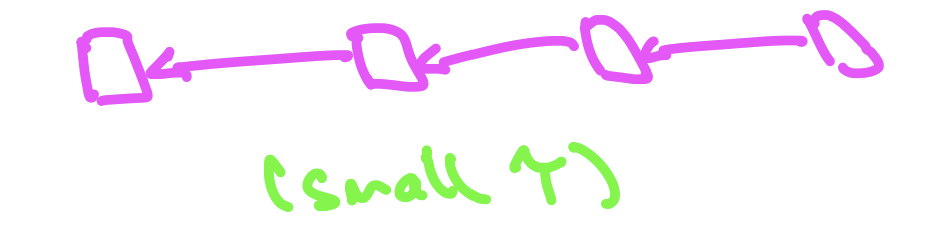
\includegraphics[width=7cm]{figures/f38.png} }}%
    \qquad
    \subfloat[]{{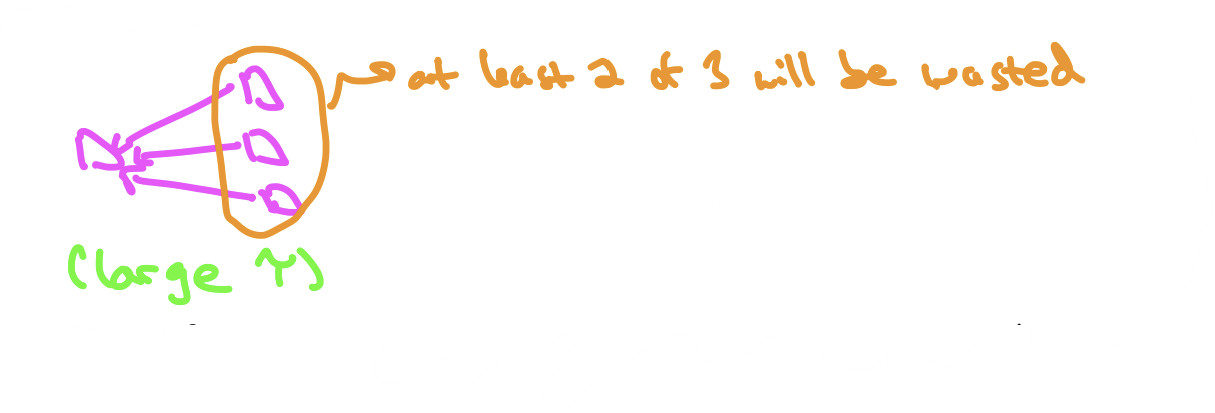
\includegraphics[width=7cm]{figures/f39.png} }}%
    \caption{}
    \label{fig:example}%
\end{figure}\\

Honest nodes are vulnerable to inadvertent forks if the time it takes for them to communicate can exceed the length of a round (with the second node succeeding before hearing
about the first node’s success). We haven’t had to discuss such forks thus far in this chapter,
but that’s an artifact of our convenient but unrealistic assumption (A5) that we’re working
in the super-synchronous/instant-communication model. In this model, all honest nodes
effectively communicate by telepathy and learn instantaneously about any newly created
blocks by honest nodes and immediately switch to trying to extend the latest one. Thus,
inadvertent honest forks are impossible in this model, no matter how quickly blocks are
created (i.e., no matter how easy the puzzles are, no matter how large $\tau$ is).\\

\noindent
\textbf{Summary.} The difficulty parameter $\tau$ should be set to balance two competing goals: (i)
a reasonably fast block rate; and (ii) a reasonably low frequency of inadvertent forks caused
by honest nodes on account of outdated information.
Working with assumption (A5) suppressed consideration (ii), which is why the value of $\tau$
has not mattered in any of our analyses so far. Section 9.7 relaxes assumption (A5) and extends
all of our provable guarantees for longest-chain consensus to the standard synchronous model
(with some known maximum message delay $\Delta$). In that section, we’ll learn that, in order to
keep the rate of inadvertent honest forks under control (and thereby preserve our consistency
and liveness arguments), the difficulty parameter $\tau$ should be set so that the typical length
of a round (i.e., the typical time between successive puzzle solutions) is larger than $\Delta$ by
a constant factor (e.g., somewhere between 5 and 100, depending on how conservative you
want to be). So, how should the parameter $\tau$ be set?
\nt{
\begin{center}
    \textbf{How to Set $\tau$}
\end{center}Set the difficulty parameter $\tau$ to target a desired rate of block production,
which in turn should be a constant factor larger than the maximum message
delay.}
One approach to tuning the constant would be to set a maximum tolerable orphan rate (e.g.,
10\%) and take $\tau$ (and hence the block rate) as large as possible subject to this constraint.
\subsection{Case Study: Bitcoin}
Nakamoto anticipated that the amount of hash rate participating in the Bitcoin protocol
could vary widely over time (due to Moore’s law, the increasing popularity of the protocol,
etc.) and, famously, that protocol tunes its difficulty adjustment parameter $\tau$ to target the
production of on average one block per ten minutes (6 blocks an hour, 144 blocks a day, 1008
blocks a week). This is a relatively conservative target, perhaps two orders of magnitude
larger than typical message delays over the Internet.\\

One, just because the popularity of the protocol could vary over time, but also because
of technological advancements, Moore’s law, etc. That would also be a force causing
hash rates to increase as time goes on. Hopefully, it’s intuitively clear that if you want to
keep the rates of block production, in other words, the frequency with which puzzles get
solved, if you want that to remain roughly constant, even as the hash rate fluctuates, well,
you better make sure that the threshold tau fluctuates in the same way.
To maintain this target rate of block production, the Bitcoin protocol must adjust the
difficulty parameter to offset changes in the hash rate (e.g., if the hash rate doubles, $\tau$ should
be cut in half). In mode detail, whenever 2016 new blocks have been added to the longest change, the protocol updates $\tau$. Note that 2016 is the target number of blocks for a fortnight
(two-week period). So the protocol looks and how long it actually took for the longest chain
to grow by this amount. If it took longer than expected (e.g., four weeks instead of two) the
puzzle difficulty is adjusted accordingly (e.g., doubling $\tau$ ). Similarly, if those 2016 blocks
were added over the course of only one week, then the protocol would halve the difficulty
parameter. In general, if it took $\beta$ · 14 days to add 2016 new blocks to the longest chain, the
difficulty parameter $\tau$ gets multiplied by $\beta$. (This formula ensures that, if the hash rate stays the same, then future blocks will be created on average
once per 10 minutes. Taking this approach means that $\tau$ is a lagging indicator of the overall hash rate; the hash rate
has for the most part been increasing over time and as a result, the average rate of block production has
generally been a little faster than one per ten minutes)

\subsection{The Role of Block Timestamps}
If you’ve been paying close attention, you might be puzzled by the preceding description of
Bitcoin’s difficulty adjustment mechanism. In Section 9.5.4 we mentioned that one remarkable
property of Nakamoto consensus, as opposed to the permissioned and proof-of-stake implementations of longest-chain consensus, is its lack of reliance on a global shared clock. This
property follows from the event-driven nature of Nakamoto consensus (with rounds delineated by new puzzle solutions), as opposed to the time-driven approach of other longest-chain
consensus implementations.
Meanwhile, in Bitcoin, the difficulty adjustment algorithm measures the amount of (real world) time that elapsed during the addition of the most recent 2016 blocks on the longest
chain. How does the Bitcoin protocol know what time it is? Isn’t the Bitcoin blockchain
supposed to act as a hermetically sealed environment?
The one concession the Bitcoin protocol makes to acknowledging the outside world is
that every block is required to include a timestamp (in addition to transactions, a pointer to
a predecessor block, and other block metadata), precisely so that the difficulty adjustment
algorithm has the information that it needs. A block’s timestamp is set by its producer.
(Honest) nodes running the protocol are supposed to include accurate timestamps, and also
to enforce some rules around timestamps so that they can’t be manipulated too much by
Byzantine nodes. (Because the timestamps play no role other than measuring the elapsed
time every 2016 blocks, minor timestamp manipulations have a negligible effect on the protocol.) The details of these rules are way out in the Bitcoin weeds (and arguably the least
elegant aspect of the protocol’s design), so for this chapter, we’ll just assume that all blocks
come with accurate timestamps. 
\subsection{Work-Adjusted Longest-Chain Consensus}
The inevitability of and complications from difficulty adjustment. With proof-of-work sybil-resistance, significant fluctuations in the overall hash rate over time seem inevitable, necessitating a difficulty adjustment algorithm to retain control over the rate of block production. While difficulty adjustment may be unavoidable, that doesn't stop it
from being annoying and leading to other problems. One example will be the next chapter
(chapter 10), in which we’ll see how deliberate forking attacks and delayed block creation
announcements can manipulate the difficulty adjustment algorithm to boost the share
of block rewards earned by a deviating node.\\
This section concerns a different issue, namely that we now need to revisit what we mean
by a longest chain. To this point, “longest chain” has meant among
all chains, the one with the largest number of hops (equivalently, the chain whose tip is farthest
from the genesis block). And this is indeed the appropriate definition for the permissioned
implementation of longest-chain consensus, as well as typical proof-of-stake implementations.
For Nakamoto consensus, this would be the appropriate definition only if the overall hash rate
stayed fixed (and, generally, it doesn't).\\

\noindent
\textbf{A bad example for naive longest chain.} To see the issue, imagine a Byzantine node
that has 10\% of the collective hash rate of the honest nodes. If all nodes attempt to produce
blocks of the same difficulty (i.e., with the same $\tau$ ), then honest nodes will create blocks 10
times as often as the Byzantine node. If the Byzantine node is only trying to create blocks
that are 100 times easier (i.e., with $\tau$ 100 times as large as that for the honest nodes),
however, then it will create blocks (of low difficulty) 10 times as often as the honest nodes
create blocks (of high difficulty). In the most extreme case, the Byzantine node could go
back to the genesis block (when the proof-of-work puzzles were incredibly easy)
and rapidly create a long chain of super-easy blocks (setting the blocks’ timestamps in such
a way that difficulty adjustment does not kick in and so puzzles remain super-easy). Were
the protocol to use the naive (unweighted) longest-chain rule, the Byzantine node might be
able to eventually create an alternative chain (of low-difficulty blocks) that is the longest chain
overall, leading to a rollback of a massive number of blocks (a big consistency/finality
violation). Various details of the Bitcoin protocol interfere somewhat with this Byzantine strategy, but this simplified example provides accurate intuition for why the protocol should weigh blocks by difficulty as opposed
to treating them all the same.\\
\qs{}{Propose a concrete strategy for a node with less than 50\% of the overall hash rate that conforms
to all of Bitcoin’s timestamping rules and leads to a consistency violation (assuming that the security
parameter $k$ is 100).}\\

\noindent
\textbf{Weighting by the amount of work.} There’s an obvious fix to this issue, which is to
weigh a block according to the amount of work that went into producing it, and then
redefine “longest chain” as the chain with the most overall weight. While we can’t know
exactly how much work (i.e., how many attempted hashes) went into the production of a
block. Only the puzzle solution is recorded, not all the failed attempts that led up to it. We
do know the expected number of hashes required to create a block with a given difficulty
threshold. For instance, with SHA-256 and a difficulty threshold of 2186, any given attempt
has a $2^{186}/2^{256} = 2^{-70}$ chance of succeeding (under the random oracle assumption), which
means that in expectation $2^{70}$ hashes must be attempted before finding a puzzle solution.
We can thus define the work of this block to be $2^{70}$. More generally, we can define the work of a block as the expected number of attempts that would be required to produce that
block. Because the work of a block is a function only of the difficulty threshold $\tau$ (which is
maintained by the protocol and its difficulty adjustment algorithm throughout its execution)
and other hard-coded parameters (e.g., the length in bits of a candidate puzzle solution), the
protocol can easily compute the work of each block. (In fact, in the Bitcoin protocol, the work of a block can be read off immediately from its metadata
(which includes the current value of $\tau$ ).) We can then define the work of a chain
as the sum of the work in each of the chain’s blocks. Honest nodes in Nakamoto consensus
are then instructed to propose only blocks that extend the highest-work chain (and, as usual,
to include all known outstanding transactions and announce the new block immediately),
without regard to the number of blocks in the chain. In the preceding example, a Byzantine
node with 10\% of the overall hash rate could still create a long alternative chain of blocks
with low puzzle difficulty, but because the total amount of work in that chain will be so low,
honest nodes will continue to ignore it.\\

\noindent
\textbf{Revisiting consistency and liveness.} We proved our consistency and liveness guarantees in chapter 8 (and extended in this chapter) for longest-chain consensus specifically for
the case of fixed difficulty and the simple block-counting definition of “longest”? Do these
guarantees carry over to general Nakamoto consensus (with variable difficulty and difficulty
adjustment) with our work-adjusted version of the longest chain rule?\\
Happily, the answer is yes, provided the following three (hopefully unsurprising) assumptions hold (in addition to standing assumptions summarized at the end of Section 9.5.2):
\nt{
\begin{center}
    \textbf{Additional Assumptions for Consistency and Liveness of
Work-Adjusted Longest-Chain Consensus}
\end{center}
\begin{enumerate}[label=(\roman*)]
    \item The security parameter $k$ is sufficiently large.
    \item At every moment in time, less than half the hash rate is controlled by
Byzantine nodes.
    \item The amount of overall hash rate changes only at a bounded rate over time.
\end{enumerate}
}

Assumption (i) we've had all along, but we’re restating it here to emphasize that, for provable
consistency and liveness guarantees, the parameter $k$ may need to be chosen somewhat
larger in the variable-difficulty case than suggested by the original fixed-difficulty analysis.
Assumption (ii) hopefully strikes you as obviously necessary—as we saw in chapter 8, if
Byzantine nodes control 51\% of the overall hash rate for a while, they can wreak
havoc (e.g., force the rollback of many blocks) through deliberate forking attacks.
The interaction between assumptions (i) and (iii). The need for assumption (iii)
may not be obvious, so let’s talk through an extreme example to develop intuition about it.
Suppose you’re happily running longest-chain consensus with security parameter $k = 100$ (say), the difficulty has stayed constant so far, and 1000 blocks have been created and added to
longest chain. The first 900 blocks on this chain are thus regarded as finalized. But now
suppose there’s a massive (billion-fold, say) increase in the overall hash rate. Now, all blocks
from the “low-difficulty period” will count for almost nothing during the subsequent “high-difficulty” period. For example, if a Byzantine node happens to be the first one to create
a high-difficulty block, and that block extends the genesis block, then all the honest nodes
(who dutifully extend the chain with the most work) will trigger a consistency violation
by abandoning the previous chain (including the 900 once-thought-finalized blocks) in favor
of extending the new high-difficulty block.32\\
\qs{}{Flesh out this example further so that it properly accounts for the lag between a hash rate
increase and the subsequent difficulty increase.
}

The role of assumption (iii), then, is to rule out such extreme (and arguably unrealistic)
examples. For example, suppose we’re willing to assume that the overall hash rate at most
doubles during any given epoch (2016 new longest-chain blocks in Bitcoin). It’s still true
that blocks produced after the doubling carry more weight than those produced before, but
only twice as much. Thus, as long as the longest chain at the time of the doubling has
a significant lead over the next-longest chain, it will still have a meaningful (though less
secure) lead after the doubling. This argument shows why the security parameter $k$ should
be set larger in the variable-difficulty setting than in the fixed-difficulty setting: a larger $k$ means that rolling back $k$ blocks is highly unlikely even after the overall hash rate doubles and pre-existing blocks count only half as much. The wilder the fluctuations in hash rate
that are allowed in assumption (iii), the bigger the increase in the security parameter $k$ that
is needed to compensate.\\

This concludes our heuristic argument that under assumptions (i)–(iii) and those at the
end of Section 9.5.2, variable-difficulty Nakamoto consensus satisfies consistency and liveness
(with high probability) even when 49\% of the hash rate is controlled by Byzantine nodes.
For a fully rigorous analysis, making precise the intuition described here, see the paper by
Garay et al. .\\


\section{Extending the Analysis to the Synchronous Model}
Section 9.5.2 reviewed the assumptions under which we proved (in Chapter 8) that longest chain consensus guarantees (probabilistic) consistency and liveness (with at most 49\% of
the hash rate controlled by Byzantine nodes). Assumption (A1) is a trusted setup assumption (no advance knowledge of the genesis block) and we’re continuing to take that on
faith. We argued there why Nakamoto consensus satisfies assumptions (A2)–(A4) (under
the random oracle assumption). That left us with the assumption (A5), our unrealistic adoption of the “instant communication” or “super-synchronous” model in which honest nodes
can communicate instantly, as if by telepathy. In addition to being patently false in any real communication network, this assumption trivialized
consistency between different honest nodes. (It did not, you’ll recall, trivialize finality, meaning an honest
node’s consistency with its future self.)
 we've promised over and over again that
all the guarantees we've proved for longest-chain consensus continue to hold (with minor
degradation) in the general synchronous model (with an a priori known bound $\Delta$ on the
maximum message delay), provided the average duration of a round (i.e., time elapsed between consecutive puzzle solutions) is larger than $\Delta$ (say, 1-2 orders of magnitude). This section, finally, supplies the math that fulfills this promise. This extension is straightforward when rounds have deterministic durations, as in typical permission
and proof-of-stake implementations of longest-chain consensus. The idea is to set the round length bigger
than $\Delta$ so that at the start of each round honest nodes can be sure to have heard about messages (like
announcements of newly created blocks) sent by other honest nodes at the beginning of the previous round.
The present setting of Nakamoto consensus, with its variable-length rounds, is the one in which non-trivial
work is required. This is also the section where,
finally, the analysis will give us concrete guidance about how to the difficulty threshold $\tau$
in Nakamoto consensus. (With assumption (A5), $\tau$ played no role in our analysis.
Here, we’ll see that it should be set to target a rate of block production.))

\subsection{Isolating the Role of Assumption (A5)}
Let’s review all our results from Chapter 8 about longest-chain consensus and examine exactly
where our proofs break down without assumption (A5).\\

\noindent
\textbf{Liveness and chain quality.} In chapter 8, under the assumption (A5), we proved that as long
as each leader of longest-chain consensus is chosen independently and has a bigger-than-50%
chance of being an honest node, then the longest chain will (with high probability) contains
blocks produced by honest nodes regularly. (Because an honest node includes all
outstanding transactions that it knows about in its block, this implies that a transaction
known to all honest nodes will eventually be included in a finalized block.)\\
The proof of this guarantee hinged on the following property:\\
\begin{itemize}
    \item Whenever there’s a round with an honest leader, the length of the longest chain known
to all honest nodes increases by one.
\end{itemize}
This follows from the fact that all honest nodes know about the same set of blocks
(under the assumption (A5)) and that an honest node extends the end of the longest chain that it
knows about. The following consequence of this property is enough for our purposes:\\

(*) the length of a longest chain known to an honest node is at least the number of blocks
that have been produced thus far by honest nodes.\\

Why was property (*) useful in the proof? Imagine that each leader has a 51\% chance of
being honest and consider the first 1000 rounds. In expectation, this sequence will have 510
honest leaders and the key property implies that the longest chain will grow in length by
at least 510 during this time. Because there were only 490 Byzantine leaders during this
time, at least 510 - 490 = 20 of the last 510 blocks on the longest chain must have been
contributed by honest nodes. In Nakamoto consensus, the leader of a given round can produce only one block and thus trivially can
contribute only one block to the longest chain. Even under the weaker assumption (A4) from Chapter 8, the
version appropriate for the permissioned and proof-of-stake implementations of longest-chain consensus, the
leader of a given round can produce multiple blocks overall but can contribute only one block to any given
chain.\\

The same argument implies a more general “chain quality” guarantee for longest-chain
consensus: if Byzantine nodes control an $\alpha$ fraction of the hash rate, then over $T$ time steps
the longest chain grows by at least $(1 - \alpha)T$ (in expectation) with at most $\alphaT$ of the growth
due to blocks produced by Byzantine nodes. That is, we expect at least a $\frac{1 - 2\alpha}{1 - \alpha}$
fraction of the blocks on the longest chain to be contributed by honest nodes.\\

\noindent
\textbf{Failure of property (*).} Property (*) breaks down when we pass from the super-synchronous
model (assumption (A5)) to the standard synchronous model with non-zero message delays
(up to a known bound $\Delta$). For example, suppose all nodes are honest and have produced
a longest chain ending with the block $B$. All the nodes then attempt to produce a block
extending the block $B$; at some point, some nodes will succeed in producing such a block $B_1$.
Because the node is honest, it will immediately announce the new block so that other nodes
can stop working to extend the tip $B$ of the old longest chain and switch to the tip $B_1$ of the
new longest chain. These announcements might take up to $\Delta$ time steps to arrive, however,
which raises the possibility that some other node will succeed in extending $B$ with a new
block $B_2$ before it hears $B_1$’s announcement (Figure 9.4). Whenever this happens (as it will,
inevitably, on occasion), property (*) is violated: two blocks get produced by honest nodes
(like $B_1$ and $B_2$) but the longest chain known to honest nodes increases by only one.
This example also provides accurate intuition for why this breakdown of property (*)
doesn't have to be a big deal. Such honest inadvertent forks occur only if two nodes solve
puzzles at almost the same time (less than $\Delta$ time units apart). As long as puzzles are typically solved infrequently (on average once every $L$ time step, with $L$ much bigger than $\Delta$),
such near-ties should be rare. Rereading the liveness and chain quality arguments above, it
would seem that they should go through as long as most (if not all) honestly produced blocks
increase the length of the longest chain. As we’ll see later in this section, this is indeed the
case.\\

\begin{figure}[h]
    \centering
    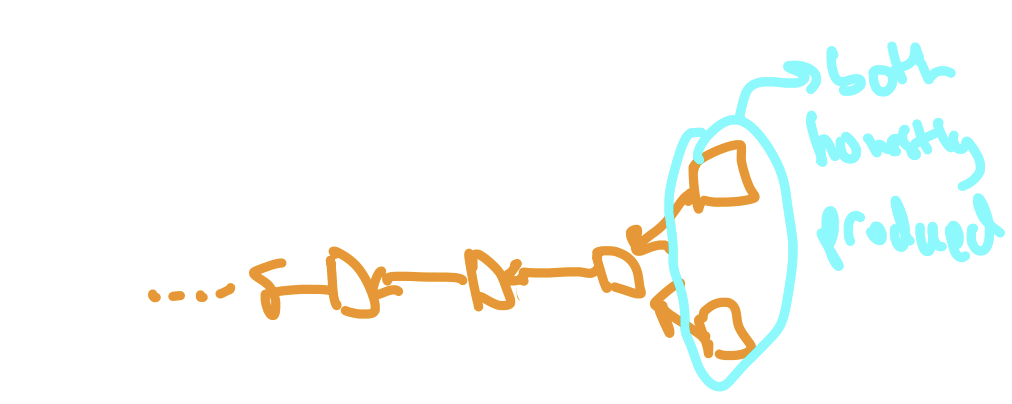
\includegraphics[scale = 0.5]{figures/f40.png}
    \caption{}
    \label{fig:mesh1}
\end{figure}\\

\noindent
\textbf{The common prefix property.} The analysis in Chapter 8 also leaned on the assumption (A5)
in its proof of the common prefix property, the property that (for a suitably large choice
of the security parameter $k$) all the longest chains known to an honest node agree except
perhaps on their last $k$ blocks. This analysis hinged on the property:\\

(**) at each block height, there is at most one block produced by an honest node.\\

Why was this property useful? Our proof of the common prefix property in Chapter 8
proceeded by contradiction, and showed that every violation of the common prefix property
must be caused by an unbalanced leader sequence (with Byzantine leaders outnumbering
honest leaders in some long window), which in turn happens only rarely when at least 51\%
of the hash rate is controlled by honest nodes. This contradiction rested on a counting
argument that established a lower bound on the number of Byzantine leaders and an upper
bound on the number of honest leaders in a long window. Property (**) gave us the latter
bound, which implied in turn the former bound. This was the argument specifically for Nakamoto consensus, using the stronger version (A4’) of assumption (A4) stating that each leader can only produce one block. As discussed in Chapter 8, a more complicated
analysis is required for permissioned and proof-of-stake implementations of longest-chain consensus, which
satisfy (A4) but not (A4’).\\

\noindent
\textbf{Failure of property (**).} A glance at Figure 9.4 shows that property (**) also
breaks down when passing from the super-synchronous model to the standard synchronous
model with non-zero message delays—if one honest node has stale information and is unaware
of a block recently produced by some other honest node, it might wind up creating a second
block at the same block height. Again, this breakdown doesn't seem a big deal as
long as such inadvertent honestly created forks are rare (which, intuitively, should be the case
if the average time $L$ between puzzle solutions is much bigger than the maximum message
delay $\Delta$). Presumably, the counting argument still works (with mildly degraded parameters)
if almost all of the blocks produced by honest nodes have distinct block heights?\\

\noindent
\textbf{Finality.} The last guarantee that we proved in Chapter 8 was (probabilistic) finality, meaning that with high probability, blocks that are at least $k$ blocks deep on the longest chain will
never be rolled back (for a sufficiently large security parameter $k$). (As always with longest chain consensus, the most recently added blocks on the longest chain should be viewed as
tentative and still under negotiation.) If we look back at the argument in Chapter 8, we’ll
see that assumption (A5) played no role, the only way to violate finality is to violate the
common prefix property. Thus, as long as we’re able to repair the proof of the common
prefix property in the standard synchronous model, we’ll immediately get finality in that
model for free.\\

\noindent
\textbf{Consistency.} Remember that for the state machine replication problem, “consistency”
means two things, consistency between different honest nodes at a given moment in time
(i.e., no two honest nodes have finalized different blocks at the same block height), and
consistency between an honest node and its future self (i.e., “finality”). The former was
trivialized by assumption (A5), with all honest nodes automatically in sync with identical
information at all moments in time. Thus, in passing to the general synchronous model, we
not only have to fix our previous proofs of liveness and the common prefix property, but we are
also now responsible for proving consistency in full. Happily, it turns out that consistency
follows from the (general version of the) common prefix property in much the same way that
finality does, so we’ll leave the details of that argument as an exercise for the reader.\\

\noindent
\textbf{Summary.} What goes wrong when you relax assumption (A5) and consider the synchronous model with non-zero message delays is the appearance of inadvertent honestly created forks (as in Figure 9.4). The hope is two-fold: first, that such forks are infrequent
as long as the typical time $L$ between puzzle solutions is sufficiently larger than the maximum message delay $\Delta$; and second, that as long as such forks are infrequent, our analysis in
chapter 8 suffer minimal damage and largely carry over. Next, we provide further details on
why both of these hopes are correct.

\subsection{ The Role of Puzzle Difficulty}
By now it is evident that two parameters (and the ratio between them) should play a crucial
role in our revised analysis:
\begin{itemize}
    \item $\Delta$, the maximum message delay (in time steps);
    \item $L$, the expected number of time steps between successive puzzle solutions.
\end{itemize}
The parameter $\Delta$ is a property of the communication network, which the protocol has no
control over. The parameter $L$, on the other hand, is determined by the protocol’s choice of
difficulty parameter (and by the current amount of overall hash rate). That is, the protocol is
in a position to choose $L$ however it wants, by setting the difficulty threshold $\tau$ appropriately.\\

To explain, suppose the amount of overall hash rate is fixed, with nodes collectively capable of $H$ attempts at puzzle solutions per time step. By the random oracle assumption,
each of these attempts has the same probability $p$ of succeeding. (E.g., in the usual case
of SHA-256 and $\tau = 2^{186}$, $p = \frac{2^{186}}{2^{256}} = 2^{-70}$.) Then, in each time step, the probability
that a puzzle solution is found (and a new round starts) is well approximated by $Hp$. For
example, if $H = 2^{50}$ and $p = 2^{-70}$, then the chance of some node finding a puzzle solution in
any given time step is roughly one in a million. This approximation applies when $H$ is small, in which case the probability that more than one solution
is found in the same time step is negligible and can be safely ignored. The story is similar when Hp is not
small, just with somewhat less convenient formulas.
The expected duration of a round—the expected number of time steps that elapse before a new solution is found—equals the expected
number of flips of a coin with bias Hp needed to see “heads.” This is a geometric random
variable (see footnote 18), with expectation of $1/Hp$. In our running example (with $H = 2^{50}$
and $p = 2^{-70}$), we should expect to see a new puzzle solution on average every million or so
time steps. If each time step represents one millisecond, say, then the average duration of a
round would be roughly 1000 seconds (1$16 \frac{2}{3}$ minutes).
In general, for the case of an SHA-256-based crypto puzzle, the average duration $L$ of a
round satisfies
$$L = \frac{1}{Hp} = \frac{2^{256}}{H.\tau}$$
Thus, for any fixed hash rate H, the protocol can target a desired rate of block production
by setting $\tau$ appropriately ($\tau = \frac{2^{256}}{HL}$). In other words, once a policy decision has been
made about the right choice for the average round length $L$, the target of the protocol’s
difficulty adjustment algorithm is uniquely determined. And how should this policy decision be made? As we’ll see below, it’s wise to choose $L$ to that $\Delta/L$ is reasonably small (e.g., at most 0.1). And how should you decide on an appropriate value for the worst-case message delay $\Delta$? That depends
on the communication network and its reliability. For a geographically concentrated and well-connected set
of nodes, perhaps $\Delta$ could be taken as a few hundred milliseconds. For nodes scattered across the globe
communicating over the Internet, $\Delta$ might be an order of magnitude larger.

\subsection{Safe Blocks}
In Section 9.7.1 we built intuition for the hope that, as long as inadvertent forks by honest nodes
(due to two puzzles found at nearly the time) are infrequent, our analysis from Chapter 8
should carry over with minimal loss. The next step is to analyze just how infrequent such
forks are, as a function of our two key parameters, the maximum message delay $\Delta$ and the
average length $L$ of a round.
The definition of safe blocks. To motivate the next definition, think about an honest
node that successfully finds a puzzle solution at some time step $t$, resulting in a new block
that extends the longest chain that the node knew about at that time. The worry is that
the node had stale information about the longest chain and was therefore doing redundant
work, creating a fork rather than extending the true longest chain (as in Figure 9.4). Because
honest nodes announce newly created blocks immediately and these announcements cannot
get delayed more than $\Delta$ time steps, this worry can only materialize if some other honest
node successfully found a puzzle solution at one of the time steps $t = t-\Delta+1, t-\Delta+2, \cdots, t$.
We’ll call a block safe if it is produced by an honest node at some time t and it
is the only such block produced at any of the time steps $t = t - \Delta + 1, t - \Delta + 2, \cdots, t$.
Properties of safe blocks. While properties (*) and (**) don’t hold in general in the
synchronous model (Figure ??), they do hold for safe blocks (because an honest node is
always up to date on safe blocks when it creates a safe block).\\

\mprop{Honest Blocks Having Increasing Heights}{The heights of safe blocks
are strictly increasing over time.}
\begin{myproof}
Suppose that safe blocks $B_i$ and $B_j$ are produced by (honest) leaders $i$ and $j$. There’s
only one leader per round, so one of $i$ or $j$ is chosen as a leader first—let’s say $i$, with its
block $B_i$ at height $h$. Because $i$ is honest, it announces its block $B_i$
immediately, and this
announcement reaches node $j$ at most $\Delta$ time steps later. Because there are at least $\Delta$ time
steps between different safe blocks (by definition), this announcement reaches $j$ prior to the
time step in which it creates its block. Thus, because $j$ is honest, $B_j$ will extend one of
the longest chains that $j$ is aware of at the time. Because $j$ is aware of a block at height $h$
(namely, $B_i$) at that time, its block $B_j$ will have height at least $h + 1$. 
\end{myproof}

Because the length of a longest chain equals the maximum height of a block, Proposition 9.7.1 implies that the length of a longest chain is at least as large as the number of safe blocks that have been produced (the analog of property (*), with safe blocks playing the
previous role of honestly produced blocks). Proposition 9.7.1 also immediately implies that
there is at most one safe block at each block height (the analog of property (**)).\\

\noindent
\textbf{Fraction of blocks that are safe.} We can classify blocks into three types: safe (and
hence produced by an honest node), produced by an honest node but unsafe, and produced
by a Byzantine node. In the analysis below, we’re going to play it safe and treat
unsafe blocks as if they were produced by Byzantine nodes. Thus, it had better be the case
that most of the blocks produced by honest nodes are safe rather than unsafe. The next
lemma quantifies the extent to which this is true.
\mlemma{}{
$$(1 - \alpha).(1 - \frac{\Delta}{L})$$
fraction of blocks are safe.}

The point is that, as long as $L$ is large relative to $\Delta$, the fraction of safe blocks is almost
as large as $1 - \alpha$, which was the fraction of honest blocks in our original analysis (under
the assumption (A5)). Because properties (*) and (**) hold for safe blocks, that original analysis
should hopefully carry over without much trouble (details to follow in the next section).
In other words, if Delta’s small relative to $L$, we have the same thing as before basically
just with a little bit of loss. The proof, it’s not hard. It’s just really some simple probability,
so what I want you to think about, I want you to think about zooming in on a moment
in time where some node, maybe honest, maybe Byzantine, some node comes up
with a new puzzle solution. What we’re going to be interested in is the probability that that
particular puzzle solution results in the creation of a safe block.\\

\noindent
\textit{Proof of Lemma 9.7.1:} Zoom in on a time step $t$ at which some block is created by some
node. For this block to be safe, two things much be true: the node producing it must
be an honest node, and no other puzzle solutions were found in any of the times steps
$t - \Delta + 1, t - \Delta + 2, \cdots, t$. That is:

$$\textbf{Pr}[\text{puzzle solution creates safe block}] = \textbf{Pr}[\text{solution found by honest node}] \times
\textbf{Pr}[\text{no puzzle solutions in last $\Delta$ time steps}]$$
Under our usual assumptions about proof-of-work (random oracle assumption, with nodes searching for
puzzle solutions by brute force), these two events are independent and so no conditioning is necessary.\\
By the sybil-resistance of proof-of-work (Theorem 9.5.1), we know that the first term on the
right-hand side equals the fraction of hash rate controlled by honest nodes (i.e., $1 - \alpha$).\\
What about the second term? Because the average duration of a round is $L$, and the
duration of a round is a geometric random variabl with parameter $\frac{1}{L}$ (see
Section 9.7.2)—the probability of a solution in any given round is $\frac{1}{L}$. Thus, the probability of a solution at any of the $\Delta$ relevant time steps
$\{t - \Delta + 1, t - \Delta + 2, \cdots, t\}$ is at most $\frac{\Delta}{L}$. This follows by the Union Bound, which states that the probability of the union of a collection of events is no larger than the sum of their individual probabilities. We last encountered the Union Bound in
chapter 8, when analyzing the balancedness properties of random leader sequences.
The probability of the complementary event which is the second term on the $R.H.S.$ is therefore at least $(1 - \frac{\alpha}{L})$.
\\

\subsection{Updating the Analysis}
Analyzing Nakamoto consensus appears harder in the synchronous model than the super synchronous/instant-communication model because there are now three types of blocks
rather than two. As usual (by Theorem 9.5.1), we expect an $\alpha$ fraction of the blocks to
be produced by Byzantine nodes and a $1 - \alpha$ fraction by honest nodes. In the latter group,
we expect (by Lemma 9.7.1) unsafe blocks to contribute at most a $(1 - \alpha)(\Delta/L)$ fraction of
the total blocks and safe blocks at least a $(1 - \alpha)(1 - (\frac{\Delta}{L}))$ fraction.
Unsafe blocks can’t be counted on to advance any of our goals, so the simplest and most
conservative approach is to treat them as if they were controlled by Byzantine nodes. (A
Byzantine node always has the option of acting as if it were honest, so this approach can
only make our guarantees stronger.) If you’re thinking in terms of the H’s and A’s of a leader
sequence (as in chapter 8), this analysis approach effectively switches some of the H’s in the
leader sequence to A’s (with a switching probability of $\frac{\Delta}{L}$).
Our original analysis of Nakamoto consensus (under the assumption (A5)) proved consistency
and liveness provided
\begin{center}
    fraction of blocks by honest nodes > fraction of blocks by Byzantine nodes,
\end{center}

or equivalently provided that $1 - \alpha > \alpha$ (i.e., $\alpha < \frac{1}{2}$).\\

In the general synchronous model, with unsafe blocks effectively switching sides (from
honest to Byzantine) to bat for the other team, we can piggyback on that same analysis
provided
\begin{center}
    fraction of safe blocks > fraction of Byzantine blocks + fraction of unsafe blocks.
\end{center}\\
By Lemma 9.7.1, this inequality holds (in expectation) if
$$(1 - \alpha) . (1 - (\frac{\Delta}{L})) > \alpha + (1 - \alpha)(\frac{\Delta}{L}) $$
or, equivalently, if
$$\alpha < \frac{1 - 2\frac{\Delta}{L}}{2 - 2\frac{\Delta}{L}} \quad (2)$$
Note that when $\Delta = 0$ we recover the $\alpha < \frac{1}{2}$
condition from the super-synchronous case.But more generally, when $\Delta$ is small relative to $L$, the condition degrades only mildly to
$\alpha < \frac{1}{2} - \delta$ for some small $\delta > 0$. Thus, provided difficulty is tuned so that $L$ is well larger
than $\Delta$, Nakamoto consensus really can tolerate nearly 50\% Byzantine hash rate.\\

\thm{Nakamoto Consensus in Synchronous Model}{Provided the assumptions at the end of Section 9.5.2 and inequality (2) hold, Nakamoto consensus satisfies (probabilistic) consistency and liveness.}
To review why Theorem 9.7.1 is true: by (2), safe blocks are produced at a higher rate than
Byzantine blocks and unsafe blocks combined. Safe blocks satisfy property (*) in Section 9.7.3,
and this property is all that is needed to carry out the liveness analysis from Chapter 8. (The chain quality guarantee from Chapter 8, based on the same argument, also carries over with mildly
degraded parameters.)
Safe blocks also satisfy property (**) in Section 9.7.3, and this is the main property needed
to prove the common prefix property as in Chapter 8. (The revised version of this property for the general synchronous model is: at all times, for every pair $i$, $j$
of honest nodes, and every choice $C_i$ and $C_j$ of longest chains known to $i$ and $j$ at that time, respectively,
the common prefix of $C_i$ and $C_j$ encompasses all but at most the last $k$ blocks of both $C_i$ and $C_j$ .) Finality (and consistency between
nodes) follows easily from the common prefix property as in chapter 8.\\

\noindent
\textbf{Interpretation for Bitcoin.} Our analysis demystifies why the Bitcoin protocol has a
10-minute block time. Going by the Bitcoin white paper, Nakamoto appeared to be
well aware of the importance of the ratio $\frac{\Delta}{L}$ for the protocol’s consistency and liveness
guarantees. It’s not clear what value of $\Delta$ Nakamoto may have had in mind for maximum
Internet delays on a typical day, but perhaps it could have been something like 10 seconds.
Nakamoto suggested tuning the proof-of-work puzzle difficulty so that the parameter L would
be 10 minutes. In this case, the ratio $\frac{\Delta}{L}$ would be under 2\% and, plugging into the formula
in (2), the protocol would satisfy (probabilistic) consistency and liveness even with 49\% (if
not 49.9\%) Byzantine hash rate.\\

Theorem 9.7.1 also lets us speculate how Bitcoin’s guarantees might degrade were we to
speed up the rate of block production (e.g., with the goal of boosting throughput). For
example, with a block time of one minute (and continuing to assume that $\Delta$ is 10 seconds),
the ratio $\frac{\Delta}{L}$ would be $\frac{1}{6}$ and, due to an increased rate of inadvertent forks created by
honest nodes, the guarantees of Theorem 9.7.1 would apply only when less than 40\% of the
hash rate is Byzantine. Ratchet up the block rate (i.e., decrease $L$) further, and still less
Byzantine hash rate can be safely tolerated.

\section{Impossibility of Consistency Under Partial Synchrony}
\subsection{The Impossibility Result and Its Consequences}
Pairing proof-of-work sybil-resistance with BFT-type consensus? In Section 9.3 we
made a big deal of the fact that sybil-resistance mechanisms (which decide who gets to
propose and vote on blocks) and consensus protocols (which decide which of the proposed
blocks get finalized and in what order) are fundamentally different things, and can be paired
up in multiple ways. For example, restricting to what are currently the most dominant
approaches to sybil-resistance (proof-of-work and proof-of-stake) and blockchain consensus
(longest-chain and BFT-type), there are four ways of pairing them together (see the grid in
Figure 9.1).[As a reminder, many but not all of the biggest “layer-1” blockchain protocols can be classified as one
of these four (or really, three) types.] Nakamoto consensus shows that longest-chain consensus pairs particularly well
with proof-of-work sybil-resistance. BFT-type consensus pairs well with proof-of-stake sybilresistance (as we’ll elaborate on in Chapter 12), essentially because the type of registration
typically required in proof-of-stake protocols enables a reduction from permissionless to permissioned consensus. There have also been successful examples of blockchains that combine
proof-of-stake sybil-resistance with longest-chain consensus (such as Cardano). What about
the fourth pairing, BFT-type consensus with proof-of-work sybil-resistance?\\

\noindent
\textbf{Extending Nakamoto consensus to the partially synchronous model?} A seemingly quite different question is whether we can improve longest-chain consensus so that
it has provable guarantees in the partially synchronous setting defined in Chapter 6 (with
arbitrary message delays up to an unknown global stabilization time GST, after which the
communication network acts as in the synchronous model with all message delays bounded
above by an a priori known parameter $\Delta$).\\
A brief review: BFT-type SMR protocols like Tendermint (chapter 7) typically satisfy
consistency (always) and eventual liveness (meaning liveness soon after GST passes). Guaranteeing consistency even under attacks and outages (i.e., pre-GST) is the reason why, in
Tendermint, we forced nodes to assemble (two stages of) supermajority quorum certificates
before finalizing a block.\\

With longest-chain consensus, meanwhile, consistency breaks down badly in the partially
synchronous model, even when all of the nodes are honest. (we've proven lots of nice
guarantees about longest-chain consensus, but they've all been in the synchronous model.)
The argument is simple (Figure 9.5): imagine a network partition (in the spirit of the CAP
theorem from chapter 6), with two groups of nodes and all intergroup messages delivered
immediately and all intragroup messages delayed until GST. The nodes of each group will
extend the longest chain known to them, resulting in two parallel chains growing for the
duration of the network partition. No matter what the value of the security parameter $k$ in
longest-chain consensus, provided the network partition goes on long enough (and remember,
GST can be arbitrarily large), and the two groups of nodes will finalize conflicting blocks. This is
a violation of consistency, and when the network partition ends, the group of nodes with the
shorter longest chain will be forced to roll back several thought-to-be-finalized blocks. Is
there any way we can add a little complexity to longest-chain consensus to avoid consistency
violations in the partially synchronous model?
An impossibility result. Next, we’ll prove an impossibility result that shows both why
coupling proof-of-work sybil-resistance with BFT-type consensus is a bad idea, and why
all Bitcoin-like protocols are doomed to consistency violations in the partially synchronous
model. Here’s the formal statement:
\thm{A Blockchain CAP Theorem}{Even without any Byzantine nodes,
no blockchain with proof-of-work sybil-resistance satisfies both:\\
\noindent
(1) liveness in the synchronous setting (even with $\Delta = 0$); and\\
\noindent
(2) consistency in the partially synchronous setting.}

\begin{figure}[h]
    \centering
    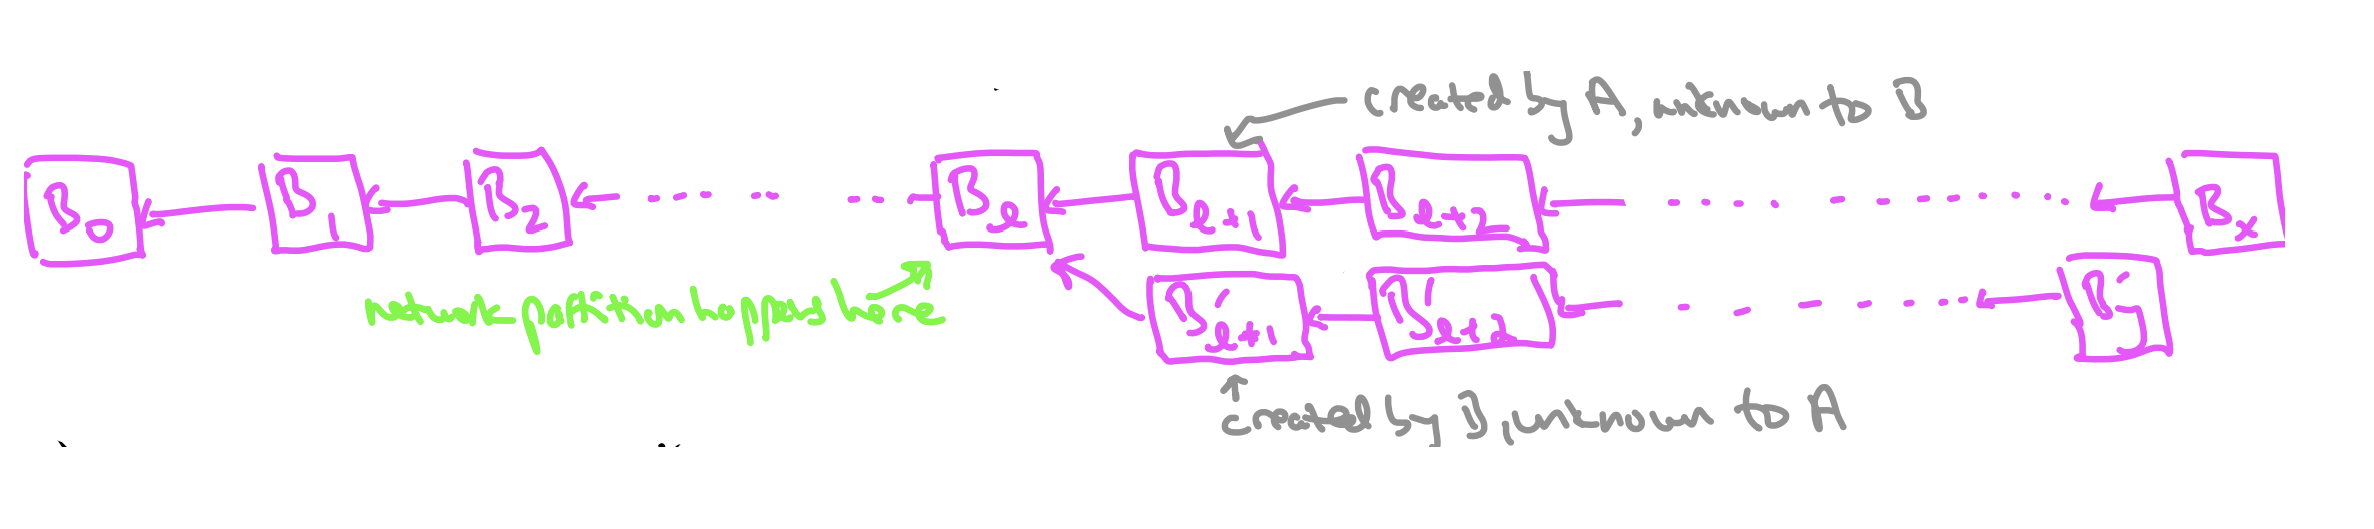
\includegraphics[scale = 0.5]{figures/f37.png}
    \caption{With a network partition, the two sides of the partition (group A and group B)
independently create two competing chains.}
    \label{fig:mesh1}
\end{figure}\\

By virtue of using proof-of-work sybil-resistance and satisfying
liveness in the synchronous model (Theorem 9.7.1), The Nakamoto consensus must necessarily suffer consistency violations in the partially synchronous model. (We already knew this via a direct argument;
the point here is that knowing nothing about Nakamoto consensus other than that it uses
proof-of-work sybil-resistance and is live in the synchronous model is already enough to automatically conclude that it cannot guarantee consistency in the partially synchronous model.)
More generally, Theorem 9.1 implies that any modification of Nakamoto consensus (e.g., as
seen in Bitcoin) that retains two of its essential properties (proof-of-work sybil-resistance and
guaranteed liveness in the synchronous model) is doomed to suffer consistency violations in
the partially synchronous model. This answers the second question above in the negative.\\

As for the first question, imagine that we attempt to couple proof-of-work sybil-resistance
with a BFT-type consensus protocol like Tendermint. This could be done in a variety of
ways, but let’s focus on couplings that preserve Tendermint’s guaranteed consistency in the
partially synchronous model. For example, one could imagine using proof-of-work sybil-resistance to randomly select a committee of nodes (with sampling probability proportional
to hash rate) and task that committee with carrying out some number of rounds of the Tendermint protocol. Assuming the sampled committees are at least two-thirds honest—which
would be true (with high probability) provided more than two-thirds of the total hash rate is
honest and the target committee size is sufficiently large. This approach would inherit Tendermint’s guaranteed consistency in the partially synchronous model. Theorem 9.8.1 would
then imply that this seemingly reasonable protocol fails liveness, even in the safe confines
of the synchronous model and with no Byzantine nodes. It’s hard to imagine deploying a
blockchain protocol that doesn't satisfy even the most basic liveness guarantees, so it’s not
surprising that we have seen any protocols of this type in the wild.\\

\noindent
\textbf{Escaping impossibility via proof-of-stake.} We’ll see in chapter 12 that Theorem 9.8.1
does not apply to proof-of-stake blockchain protocols; properly implemented, such a protocol
can satisfy liveness and consistency guarantees comparable to a permissioned protocol like Tendermint. We’ll also see that proof-of-stake blockchain protocols have some other issues. They are in some sense “less permissionless” than proof-of-work protocols and also suffer from
some additional attack vectors (such as “long-range attacks”).

\subsection{Informal Proof of Theorem 9.8.1}
The one-sentence summary of why Theorem 9.8.1 is true is that, in a proof-of-work blockchain
protocol, honest nodes cannot distinguish between a waning hash rate and delayed messages.
Note that even without any Byzantine nodes, the (honest) hash rate can fluctuate arbitrarily.
Likewise, in the partially synchronous model, messages can be delayed arbitrarily even when
there are no Byzantine nodes.\\

Concretely, zoom in on an honest node $i$ and suppose that, at some point in time, it stops
hearing any new messages from any other nodes. Two possible explanations (even without
resorting to Byzantine nodes) are:\\
\begin{enumerate}[label=(\roman*)]
    \item all other (honest) nodes turned off their machines (i.e., there’s no other hash rate in
the system);
    \item it’s pre-GST in the partially synchronous model and all messages sent by all other
(honest) nodes have been delayed (e.g., due to a network outage).
\end{enumerate}

You have to pity poor node $i$ at this point, as it’s stuck in a catch-22 and has only two options:
Either it eventually finalizes an additional block, despite not hearing from any other nodes,
or it waits (possibly forever) to finalize further blocks until it hears enough messages from
other nodes.\\

If node $i$ chooses the first route (as would be the case in Nakamoto consensus) in order
to preserve liveness but the reason for silence happens to be (ii), then the other nodes
may well be finalizing their own (conflicting) blocks, resulting in a consistency violation. If
node $i$ chooses the other option (as it would if following the Tendermint protocol), a problem
arises in scenario (i): with no other nodes to hear from, node $i$ would wait forever and no
further blocks would ever be finalized (a violation of liveness, even in the synchronous (and
even $\Delta = 0$) model).\\

Why doesn't the same argument apply to proof-of-stake protocols, in which nodes are
sampled with probability proportional to the amount of stake (in the blockchain’s native currency) that the nodes have placed in escrow? Because stake is directly observable (recorded right there on the blockchain, in plain view) while hash rate is not (e.g., you cannot definitively deduce the current amount of hash rate from the state of a proof-of-work blockchain protocol). While node $i$ in the proof above can’t know if all other nodes suddenly turned
off their machines, it would know immediately if all other nodes suddenly withdrew their
stakes. That is, the analog of scenario (i) above can be detected without any communication between nodes in a typical proof-of-stake blockchain protocol, and this fact derails the argument above.

\section{A Look Ahead to chapters 10–13}
You might be surprised that it’s possible to write and read a couple of hundred pages about
blockchain protocols without ever talking about cryptocurrencies but with chapters 1–9
that’s exactly what we've done. And indeed, while the story of blockchains and cryptocurrencies have been tightly intertwined to date (and may continue to be for a long time),
cryptocurrencies are not fundamental to blockchain protocols. As we've seen, there can
be both permissioned and permissionless blockchain protocols (with provable liveness and
consistency guarantees) without any native currency. That said, the next four chapters will
focus on blockchain protocols with a native currency, and some of the additional challenges
that come up in the design of such protocols.\\
Endowing a blockchain protocol with a native currency (with the monetary supply and
distribution managed by the protocol itself) is convenient for some reasons:\\

\noindent
\textbf{Interesting in its own right.} Perhaps the goal is in fact to create a new currency, 
a type of digital cash that can be used directly for peer-to-peer payments. Why use a
blockchain? Because blockchain protocols can be used to track digital ownership without
any centralized intermediary (under the usual assumption that a sufficiently large fraction of
the nodes/hash rate/stake is running the protocol honestly). It’s not obvious that blockchain
protocols are the only possible way to achieve this functionality, but they currently have
no real competition. It would seem that this goal was Nakamoto’s primary motivation
for inventing the Bitcoin protocol (what with the white paper’s title of “A Peer-to-Peer
Electronic Cash System”).\\

\noindent
\textbf{Incentive nodes to run the protocol correctly.} Even if you’re not trying to challenge
the US dollar or create a currency in the usual sense, a currency native to a blockchain
protocol is useful for some reasons (as the means if not the ends). For starters, in
a permissionless blockchain, why should nodes bother to run the protocol at all? There’s
only so far that a blockchain protocol can scale if relying only on altruistic or curious hobbyists. This question is particularly acute for proof-of-work protocols, given that participation
requires devoting a large amount of computation to what is otherwise useless work.\\

One natural approach is to use incentives, meaning to reward nodes for their participation
in something that has real economic value. But what could be in a protocol’s possession
that could be used as rewards to nodes? If the protocol controls a native currency, then
one obvious answer is to pay out rewards in that currency, printing new money if necessary.
(Conversely, if the protocol does not control a native currency, there’s no obvious solution
to the problem.) The protocol is in a position to print new money when needed precisely
because the currency is native to it.\\

Implementing node rewards is particularly straightforward for protocols that use longestchain consensus: every time a new block gets finalized (i.e., sufficiently deep on the longest
chain), pay a block reward to the (unique) proposer of that block. For example, the Bitcoin
protocol currently pays out 6.25 (newly minted) Bitcoins to the proposer of each finalized block. (Of course, for a reward denominated in the native currency to have meaningful economic value, the
currency itself must have some value (e.g., with people e willing to pay a non-trivial amount of fiat currency
for it). We won’t discuss here the question of when and why a cryptocurrency might have significant economic
value.)\\

If a protocol is doling out economically meaningful block rewards to nodes for producing
blocks, it’s intuitively clear that some number of people are going to be motivated to participate in the protocol and earn those rewards. But whenever you introduce incentives into a
system, you need to take a step back and ask: wait, do the rewards incentivize nodes even
more strongly to behave in other, unintended ways?\\

Chapter 10 is all about answering this question for block rewards in Nakamoto consensus.
Perhaps counterintuitively, we’ll see in that chapter that, in some settings, honestly following
Nakamoto consensus is not the profit-maximizing strategy for a node—by deviating from the
intended behavior in clever ways, a node can earn more rewards than it would otherwise!\\

\noindent
\textbf{Charge for usage.} A second convenient use of a native currency is to charge for usage.
In our chapters thus far, we've been assuming that blocks can be large enough to include
all pending transactions known to a node. As you can imagine, in practice, it’s necessary
to impose a cap on how big blocks can be. If the demand for a blockchain protocol (the
number of transactions submitted to it) exceeds its supply (the number of transactions it
can process), the protocol must decide which transactions get included and which ones get
excluded. As with any over-demanded resource, charging for usage is a natural way to limit
demand. (Even if supply exceeds demand and in principle, all transactions can be included without charging
anything, nominal transaction fees can still be a good idea (e.g., as an anti-spam measure).)\\

Implementing this idea requires a new component of a blockchain protocol that we haven’t
discussed yet, the component that decides which transactions get included and what the
creators of those transactions have to pay. This component is known as a transaction fee
mechanism and is the subject of Chapter 11.\\

\noindent
\textbf{Proof-of-stake sybil-resistance.} As mentioned many times, in chapter 12 we will explore proof-of-stake sybil-resistance, in which nodes are selected with probability proportional to the amount of money they have locked up in escrow (as opposed to the amount of
computational power that they contribute). As we’ll see, proof-of-stake sybil-resistance has
some advantages (and disadvantages) over proof-of-work, and for this reason, has become the
dominant approach to sybil-resistance in blockchain protocols over the past five years. A
proof-of-stake protocol could in principle accept stakes in some external currency (such as a
stablecoin), but it’s easier and more practical to require staking using a native currency (as
all major proof-of-stake protocols do).\\

\noindent
\textbf{Economic security.} Finally, a native currency provides a blockchain protocol with a lever
by which to control the amount of security that it provides to its users. By rewarding nodes
for participating, a protocol entices nodes to devote economic resources (computational power
or capital) to running it. Nodes incur realized or opportunity costs from such investments. The bigger the rewards, the bigger the costs that the nodes running the protocol are willing
to absorb.\\

Chapter 13 studies one definition of the “economic security” of a blockchain protocol,
roughly defined as the monetary cost that must be paid by an attacker in order to take
over the protocol (e.g., by acquiring lots of hash rate or staking a sufficiently large amount of
native currency). We’ll see in that chapter that, to first order, economic security scales with
the amount of investment by non-Byzantine nodes, which in turn scales with the economic
value of the rewards paid to the nodes running the protocol.
